\section{Introduction} 

Nucleons are the building blocks of almost all ordinary matter in the universe. The challenge of understanding the nucleon's
 structure and dynamics has occupied a central place in nuclear physics. The nucleon (proton and neutron) electromagnetic
 form factors describe the spatial distributions of electric charge and current inside
 the nucleon, hence are intimately related to its internal structure; these form factors are among the most basic observables of the
 nucleon.

Quantum chromo dynamics (QCD) is the theory of the strong interaction, which is responsible for binding quarks through the exchange of
gluons to form  hadrons (baryons and mesons). The fundamental understanding of the nucleon form factors in terms of QCD is one of
 the outstanding  problems in nuclear physics. Why do quarks form colorless hadrons with only two stable configurations, proton and neutron?
 One important step towards answering this question is to characterize the internal structure of the nucleon. High energy
 electron scattering provides one of the most powerful tools to investigate this structure. 

Early  electron scattering experiments with nuclei were motivated by a need to verify predictions of the then current models
 of the electromagnetic interaction of electrons with nuclei, and in particular with the proton and neutron; Rosenbluth
 predicted that high energy electrons would be scattered dominantly by the magnetic moment of the proton \cite{rosenbluth}. 
Available accelerators in the early fifties had energies smaller than 50 MeV, and provided much information on the nuclear
radius of elements from Be to Pb. First clear evidence that the proton was not point like was obtained at the Stanford
accelerator in the period 1953-1956, under the leadership of Robert Hofstadter. Clear demonstration that the proton has
 a finite size (unlike the electron?) had to wait for the availability of electron beams with higher energy, like
 the 550 MeV Stanford linear accelerator. In his extensive, 1956 review Hofstadter \cite{hofstadter56} discussed data
for the angular distribution of the elastically scattered electrons up to 140 degrees; these data differ from the
expectation for a point charge and magnetic distribution by a factor of five at the largest 
$ q^2= 14\times 10^{-26}\ cm^{-2}= 14 \ fm^{-2}$ or $\approx 0.73 \ GeV^2$. A proton radius of 0.77$\pm$0.1 fm was derived from
the momentum transfer squared q$^2$ dependence of a form factor $F^2(q^2)$ defined in terms of the charge density
distribution as:
\begin{equation}
\rho(r)=\frac{1}{2\pi^2r}\int F(q)sin(qr)qdq. 
\end{equation}
\noindent
In 1957 Yennie, Levy and Ravenhall \cite{yennie57} derived an expression for the ${\bf ep}$ cross section in terms of two form factors, 
$F_1$ and $F_2$, following Rosenbluth's work, as:
\begin{equation}
\sigma(\theta)=\sigma_{NS}\left\{F_1^2+\frac{q^2}{4M^2}\Big[2(F_1+F_2)^2\tan^2\frac{\theta_e}{2}\Big]\right\},
\end{equation}
\noindent
where $F_1$ was introduced to represent the spread-out charge and spread-out Dirac magnetic moment. $F_2$ describes the spread-out
Pauli (or anomalous) magnetic moment. $\sigma_{NS}$ is equal to the Mott cross section corrected for the nucleon recoil (see Eq. \ref{eq:csmott}
below). 

A similar change in accepted concepts occurred when the JLab data for the proton form factor ratio $\mu_p\frac{G_{Ep}}{G_{Mp}}$ from
double polarization experiments, completed in 2000 up to $Q^2$ of 
 5.8 GeV$^2$, differed drastically from the form factor results obtained using the Rosenbluth separation method; here $\mu_p$ is the magnetic
 moment of the proton. 
The standard data base up to this time had been entirely defined by cross section measurements, and
 suggested that, for $Q^2 < \sim 10 GeV^2$, both the electric and magnetic form factors behaved approximately like the dipole form factor:
\begin{equation}
 G_D=\Big(1+\frac{Q^2}{0.71}\Big)^{-2}, 
\label{eq:dipole}
\end{equation} 
with the four momentum transfer squared Q$^2=-q^2=-(\vec q^2-\omega^2)$; $\vec q$ the vector polarization transfer and $\omega$
 the energy transfer, in units of GeV$^2$.

What the series of experiments started in 1998 in Hall A at JLab demonstrated was that the electric and magnetic form
 factor ratio $\mu_p\frac{G_{Ep}}{G_{Mp}}$ decreased approximately linearly with Q$^2$, reaching a value of 1/3.7 times the value
 at $Q^2=0$ at the highest Q$^2$ investigated  at that time, 5.6 GeV$^2$. Coincidentally, Rosenbluth \cite{rosenbluth}
 had argued in 1950, that in a combination
of the spread-out electric charge produced by the pion cloud and the strongly anomalous magnetic moment of the proton, 
the magnetic form factor would dominate the data at large Q$^2$; fifty years later this ``prediction'' was verified by the JLab data.
And almost 60 year after the work of ref. \cite{hofstadter56} the 
question of whether the proton radius is $\approx$ 0.877 or 0.8409 fm, a difference of 6.9 standard deviations,
is being discussed intensely.

\subsection{History of elastic electron scattering on the nucleon}

Elastic electron proton scattering has evolved since the history making series of experiments with electron beams at the
 Stanford Linear Accelerator in 1956. 
Under the leadership of R. Hofstadter, a series of crucial results were obtained from cross section measurements \cite{hofs53}. 
Several fundamental pieces of information were established following these experiments, including the approximate $1/Q^8$
decrease of the cross section with the invariant four momentum transfer squared, Q$^2$, establishing the approximate shape
 of the charge distribution, and a first value for the proton radius. Theoretical
work evolved in parallel with these experimental ``firsts'', leading to the description of the elastic electron scattering
 process in terms of the lowest order process,  the exchange of a single virtual
photon with negative invariant mass squared; this lowest order contribution, also called the Born term, was expected to be dominant
 because of the smallness of the electromagnetic coupling constant $\alpha_{EM}$.  Fundamental expressions for the hadronic current
 and the definition of two invariant
form factors, $F_1$ and $F_2$, later named the Dirac and Pauli form factors, of the Born (single photon exchange) term, were issues
 of this period. Experimenters use preferably the Sachs form factors $G_{E}$ and $G_{M}$, which are linearly related to $F_1$ and $F_2$
\begin{eqnarray}
G_{E_{p,n}}& = & F_{1_{p,n}}-\tau F_{2_{p,n}} \nonumber \\
G_{M_{p,n}}& = & F_{1_{p,n}}+F_{2_{p,n}},
\label{eq:gepgmp}
\end {eqnarray}
\noindent.

The possibility of observing polarization transfer, or asymmetry, for longitudinally polarized electrons, measuring either 
the polarization transferred to the recoil proton, or the asymmetry if the target proton or neutron is polarized, was
first discussed in a paper by Akhiezer et al \cite{akh1A,akh1B}. It was to be more than 20 years before such experiments, which 
require a polarized electron beam, could be performed with good accuracy. 
Further papers on double polarization experiments followed, including Akhiezer and Rekalo  \cite{akh2A,akh2B}, and Dombey \cite{dombey}.
The accidental time coincidence of the initial phase of the construction of the CEBAF accelerator at the Thomas Jefferson National
 Accelerator Facility (TJNAF) or JLab, in Virginia,
 and a paper by Arnold, Carlson and Gross \cite{arnold} about double polarization experiments, lead to an intensive program of
 nucleon form factor experiments and a significant breakthrough in our understanding of the proton structure. A series of
 double-spin experiments, first for the proton and then for the neutron, followed, with conundrum changing consequences. 

In the Born  approximation the transferred polarization has only two components, both in the 
reaction plane defined by the beam and scattered electron, one along the recoil proton momentum, and the other perpendicular to it.
For the proton, polarization transfer has been used most often at JLab for the proton; it requires a re-scattering of the proton to
 measure its polarization, 
and is dependent on the analyzing power of the reaction used. For the neutron, target asymmetry has now been used successfully
\cite{riordan:2010} for the determination of the $G_{En}/G_{Mn}$ ratio; this requires a polarized target of either D$_2$ or He$^3$, 
which limits the maximum electron current that can be
 tolerated without significant depolarization of the target. Recent progress in the design and construction of polarized liquid
 $^3$He-target \cite{dolph:2011} indicates that future experiments on the neutron form factors should benefit of much increased beam luminosity
 (at Mainz and JLab). Solid polarized proton targets also reach high polarization by Dynamic Nuclear Polarization, but suffer
 from beam current limitations, which mitigate some of their advantage over liquid $^3$He target  because of the absence of
 nuclear effects.  

Among the earliest ${\it ep}$ published polarization experiments, a search in 1963 at the Saclay Linear Accelerator with a beam 
of 950 MeV electrons, for a symmetry 
breaking induced recoil polarization perpendicular to the scattering plane, for unpolarized beam electrons and unpolarized target protons, 
may well have been the first polarization experiment ever performed. Such an effect would be due to the interference of the Born
 amplitude with the two-photon exchange amplitude in elastic {\it {ep}} scattering. The asymmetry obtained in the vertical plane
at Q$^2$=0.61 GeV$^2$ was 0.040 $\pm$ 0.027 \cite{bizot}.

A similar single-spin experiment in 1970 with an un-polarized 15-18 GeV electron beam at the Stanford linear accelerator,
 and a polarized proton target with polarization perpendicular to the reaction plane to characterize the interference of
 the two-photon exchange with the single photon exchange (Born) process, produced asymmetries of order 0.5\% in the
 range of $Q^2$ 0.38 to 0.98 GeV$^2$. 

The early nineties saw a number of double polarization experiments at NIKHEF \cite{passchier} and MAMI \cite{herberg,ostrick} to determine 
the neutron electric form factor up to 
Q$^2\sim $1 GeV$^2$. All used polarized electron beams and a polarized target, either deuterium or $^3He$.  

The next step was the measurement of the transverse, in plane recoil proton polarization $P_t$ (or $P_x$) for longitudinally 
polarized electrons and unpolarized target in the mid nineties, at the Mainz Microtron (MAMI) \cite{eyl:1995,pospischil}. 
This experiment measured the proton form factor ratio $G_{Ep}/G_{Mp}$ up to $Q^2$ of 0.5 GeV$^2$, and the results were in agreement 
with the dipole form factor, $G_D=(1+\frac{Q^2}{0.71})^{-2}$. 

The start in 1998 of the recoil polarization program at JLab, both for the proton and the neutron, was preceded by experiments at the BATES
 Linear Accelerator. For the neutron, the pioneering experiment of Madey et al. performed the first
 recoil polarization measurement of $G_{En}$ at BATES at a Q$^2$ of 0.255 GeV$^2$ in 1994 \cite{eden:1994}. 
 For the proton the two polarization transfer components P$_{\ell}$ and P$_t$, and the corresponding
 $G_{Ep}/G_{Mp}$ ratio were measured at Q$^2$ of 0.38 to 0.50 GeV$^2$\cite{barkhuff,milbrathA,milbrathB}. 

In 2000 the SAMPLE collaboration obtained the vector analyzing power for 200 MeV transversally polarized electrons for the unpolarized proton, 
which is parity conserving and 
time-reversal odd, and tests the contribution of two-photon exchange. When compared with the results of Ref. \cite{bizot}, such transverse effects 
are suppressed by the relativist boost parameter $\gamma$. A value of  $A=-15.4\pm 5.4 \ {ppm}$ at Q$^2$=0.1 GeV$^2$ was observed
in this experiment \cite{beise:2004}. 
+
\subsection{Dirac and Pauli form factors}

The lowest order approximation for electron nucleon scattering is the single virtual photon exchange process,
or Born term. The Born approximation is expected to provide a good lowest order description of elastic $eN$ scattering (with $N=p,n$) because
 of the weak electro-magnetic coupling of
the photon with the charge and the magnetic moment of the nucleon. The amplitude for the process is the 
product of the four-component leptonic and hadronic currents, $\ell_{\nu}$ and ${\mathcal J}_{\mu}$, and
can be written as:
\begin{eqnarray}
i{\mathcal M}&=&\frac{-i}{q_{\mu}^2}\ell_{\mu}{\mathcal J}^{\mu} \nonumber \\
&=&\frac{-ig_{\mu\nu}}{q_{\mu}^2}\left[ie\bar{u}(k')\gamma^{\nu}u(k)\right]\left[-ie\bar{v}(p')\Gamma^{\mu}(p',p)v(p)\right]
\end{eqnarray}
where $k,k',p,p'$ are the the four-momenta of the incident and scattered, electron and proton, respectively,
$\Gamma^{\mu}$ contains all information of the nucleon structure, and $g_{\mu\nu}$ 
is the metric tensor. To insure relativistic invariance of the amplitude 
$\mathcal M$, $\Gamma^{\mu}$ can only contain p, p' and $\gamma^{\mu}$, besides numbers, 
masses and Q$^2$.

The most general form for the hadronic current for the spin $\frac{1}{2}$-nucleon, satisfying relativistic invariance 
and current conservation, and including an internal structure is:\\
\begin{equation}
{\mathcal J}_{hadronic}^{\mu}=ie\overline{\nu}(p')\left[\gamma^{\mu}{{F_1(Q^2)}}+
\frac{i\sigma^{\mu\nu}q_{\nu}}{2M}\kappa_{j}{{F_2(Q^2)}}\right]\nu(p) \\
\label{eq:Jhadron}
\end{equation}
\noindent where $M$ is the nucleon mass, $kappa_j,\ \mbox{with}\ j=p,n$ the anomalous magnetic moment, in units of the nuclear magneton,
 $\mu_N=\frac{e\hbar}{2M}$. $Q^2=\vec{q}^{~2}-\omega^2=-q_{\mu}^{ 2}$, 
is the negative of the square of the invariant mass $q_{\mu}^2 $ of the virtual photon of negative mass squared, exchanged in the one-photon 
approximation of $e{\it N}$ scattering. The Dirac and Pauli form factors, $F_1(Q^2)$ and $F_2(Q^2)$ are the only structure functions allowed 
in the Born term by relativistic invariance. As is now the most frequently used notation, $\kappa_jF_2\ j=p,n$ will be written as $F_{2p}$ 
and $F_{2n}$, respectively.  
In the static limit, $Q^2=0$, $F_{1p}=1$, $F_{2p}=\kappa_p=1.7928$ and $F_{1n}=0$ and $F_{2n}=\kappa_n=-1.9130$, 
for the proton and neutron, respectively.

The Lab frame differential cross section for detection of the electron in elastic $ep$ or $en$ scattering is then:
\begin{eqnarray}
\frac{d\sigma}{d\Omega_e} &=& \left(\frac{d\sigma}{d\Omega}\right)_{Mott}\frac{E_e}{E_{beam}} \Big(F_1^2(Q^2) \nonumber \\
& + & \mbox{} \tau\Big[F_2^2(Q^2) + 2[F_1(Q^2)+F_2(Q^2)]^2\tan^2\frac{\theta_e}{2}\Big]\Big)
\end{eqnarray}
\label{eq:csF2F1}
\noindent with $\tau=Q^2/4M_p^2$; $(\frac{d\sigma}{d\Omega})_{Mott}$ is the Mott cross section given by:
\begin{equation}
\left(\frac{d\sigma}{d\Omega}\right)_{Mott}=\frac{\alpha^2\cos^2\frac{\theta}{2}}{4E_{beam}^2\sin^4\frac{\theta}{2}}.
\label{eq:csmott}
\end{equation}

The incident electron (beam) and scattered electron energies are labeled $E_{beam}$ and $E_e$, respectively. The fraction $\frac{E_e}{E_{beam}}$
in Eq. \ref{eq:csF2F1} is the recoil correction to the Mott cross section Eq. \ref{eq:csmott}.

Experimental cross section data are most easily analyzed in terms of another set of form factors, the Sachs form 
factors $G_{E}$ and $G_{M}$. The relation between $G_{E}$ and $G_{M}$ and $F_1$ and $F_2$ for proton and neutron are given
 in Eq. \ref{eq:gepgmp}.
The scattering cross section Eq.~\ref{eq:csF2F1} can then be written in a much simpler form, without interference term, leading to a 
separation method for $G_{E}^2$ and $G_{M}^2$ known as Rosenbluth (or Longitudinal-Transverse) method, 
as will be seen below. Now the cross section is:
\begin{eqnarray}
\frac{d\sigma}{d\Omega_e} &=& \left(\frac{d\sigma}{d\Omega}\right)_{Mott}\frac{E_e}{E_{beam}}\frac{1}{1+\tau)} \left( G_{Ep}^2 + 
\frac{\tau}{\epsilon}G_{Mp}^2\right)
\label{eq:csgegm}
\end{eqnarray}
\noindent 
where $\epsilon$ is the polarization of the virtual photon defined as:

\begin{equation}
\epsilon=\frac{1}{1+2(1+\tau)\tan^2\frac{\theta_e}{2}}, 
\end{equation} 
\noindent 

%%%%%%%%%%Figure 1
\begin{figure}
\begin{center}
\resizebox{0.45\textwidth}{!}{%
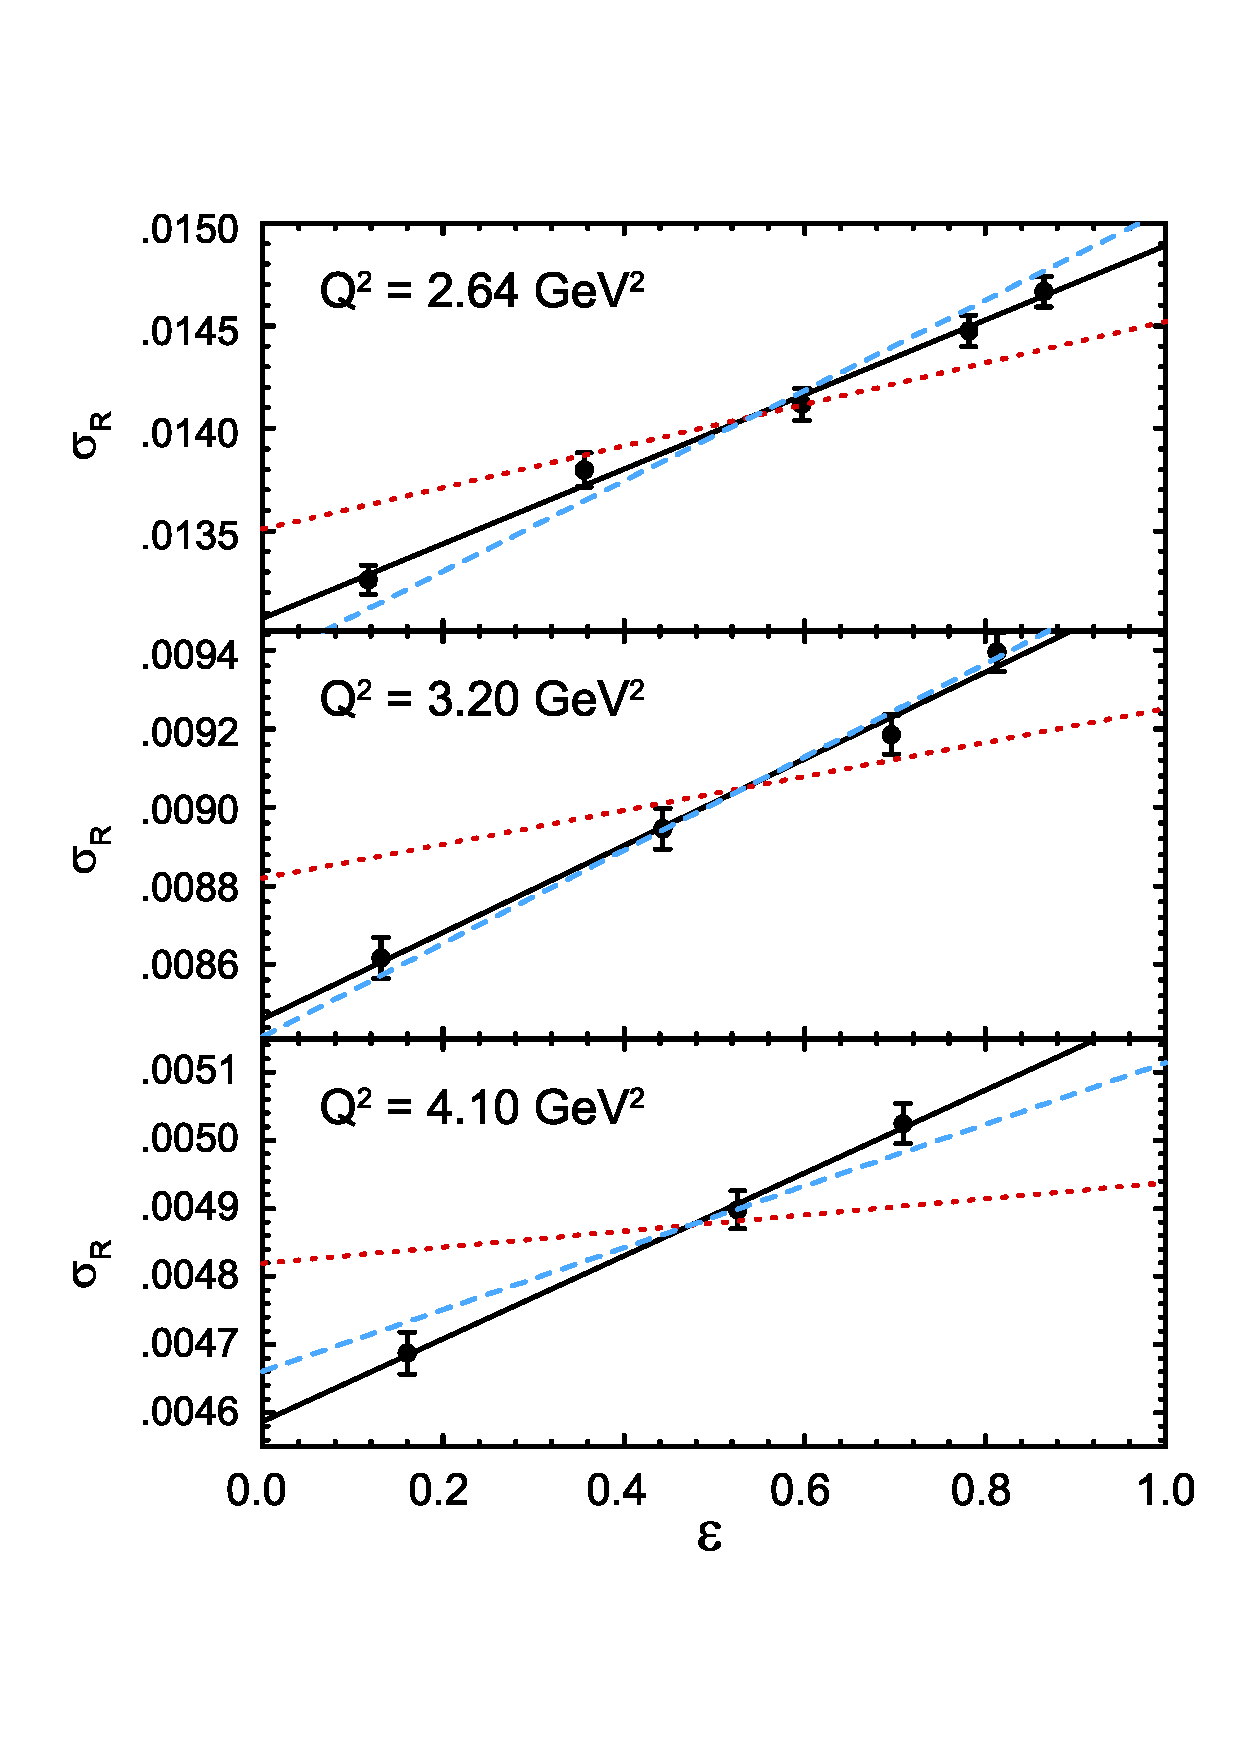
\includegraphics{FIG1.pdf}
}
\caption{Illustration of the Rosenbluth separation method to obtain separate values of $G_{Ep}^2$ and $G_{Mp}^2$ from the kinematic factor 
$\epsilon$-dependence of the reduced cross section. Data from Qattan \cite{qattan05}}
\label{fig:geplt1}
\end{center}
\end{figure}

%%%%%%%Figure 2
\begin{figure}
\begin{center}
\resizebox{0.485\textwidth}{!}{
  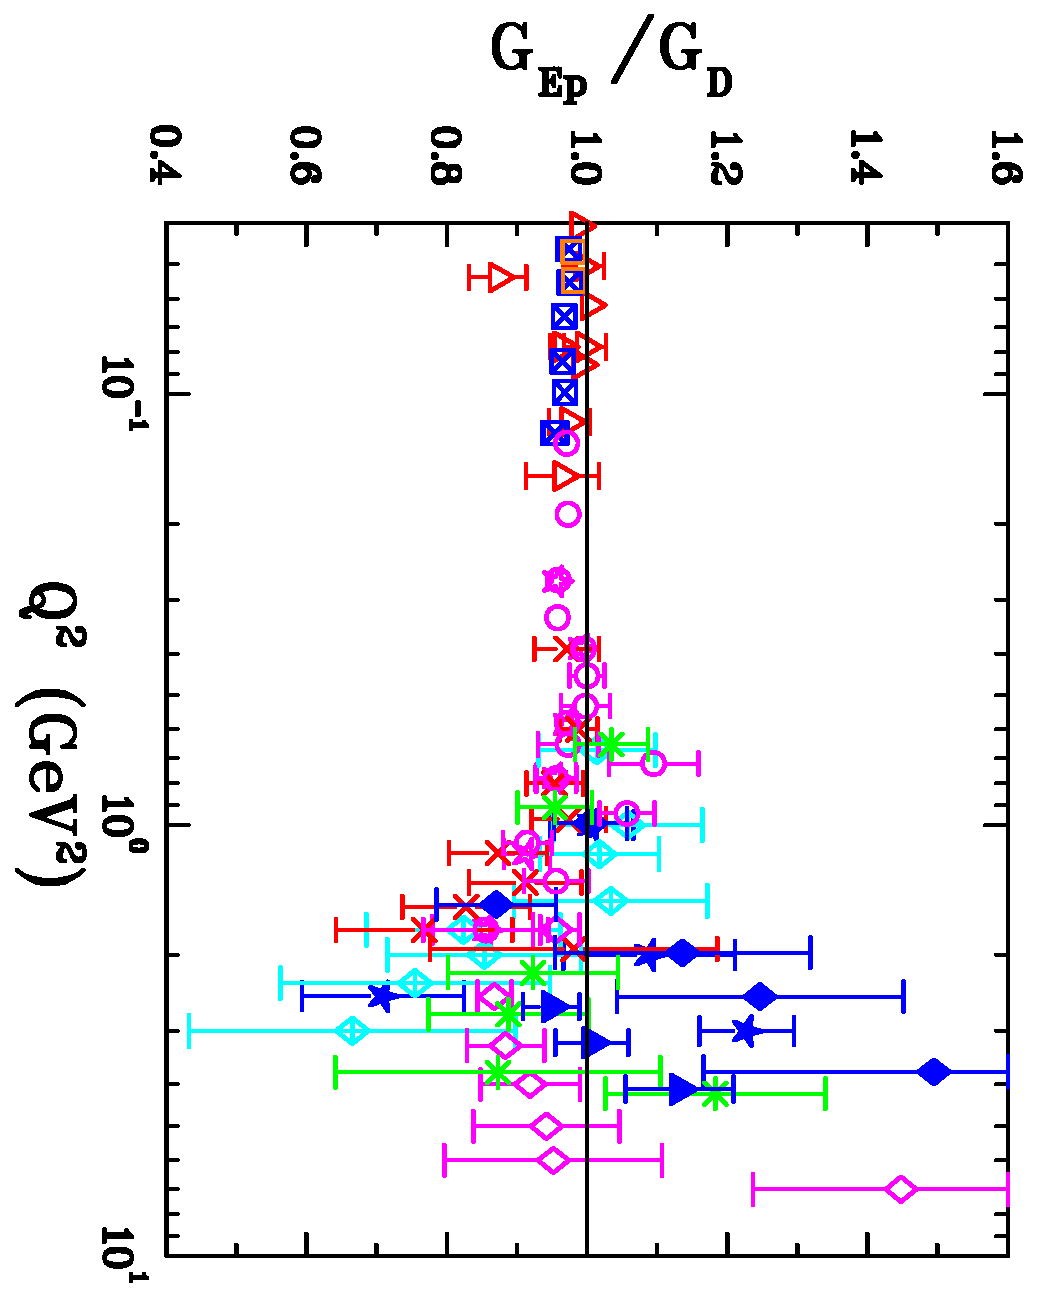
\includegraphics[angle=90]{gepgd_Dspin11.eps}
}
\caption{Q$^2$-dependence of the ratio $G_{Ep}/G_D$ obtained by the Rosenbluth separation method. $G_D$ is the dipole form factor. All data published after 1970 \cite{litt} are included}.
\label{fig:gepgd_cs}
\end{center}
\end{figure}

%%%%%%%%%%%%%%%%Fig 3
\begin{figure}
\begin{center}
\resizebox{0.485\textwidth}{!}{%
  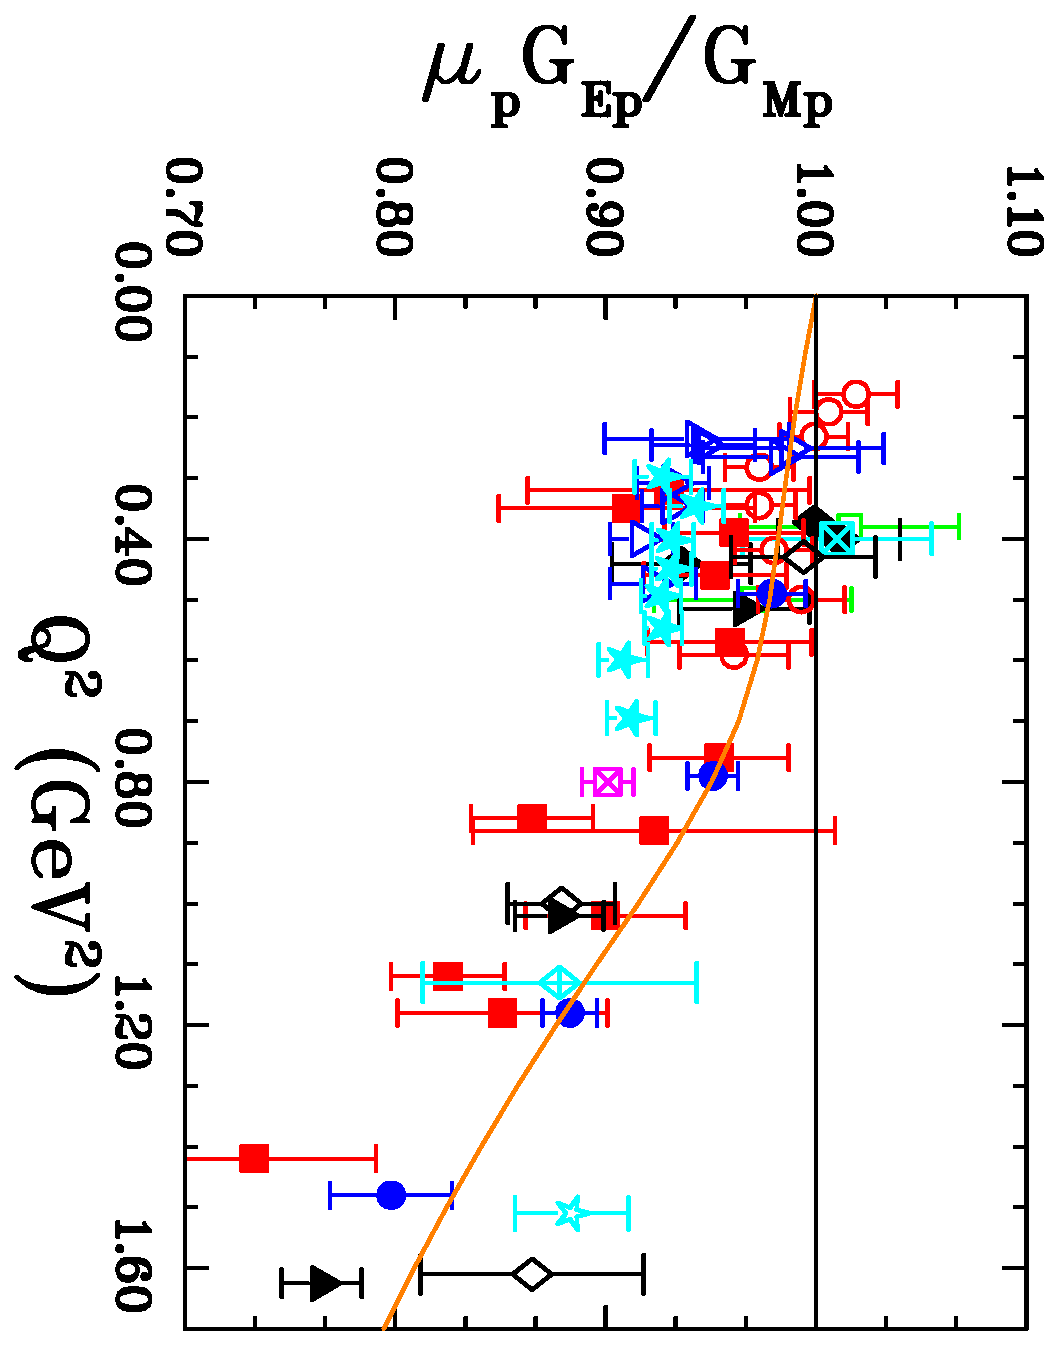
\includegraphics[angle=90]{gepgmp_low_nofit_10092014.eps}
}
\caption{Ratio $G_{Ep}G_{Mp}$ for $Q^2$ smaller than 1.5 GeV$^2$. The inconsistency of the various experiments are highlighted here.}
\label{fig:gepgmp_lowq2}
\end{center}
\end{figure}

%%%%%%%%%%%%%%Figure 4
\begin{figure}
\begin{center}
\resizebox{0.485\textwidth}{!}{%
  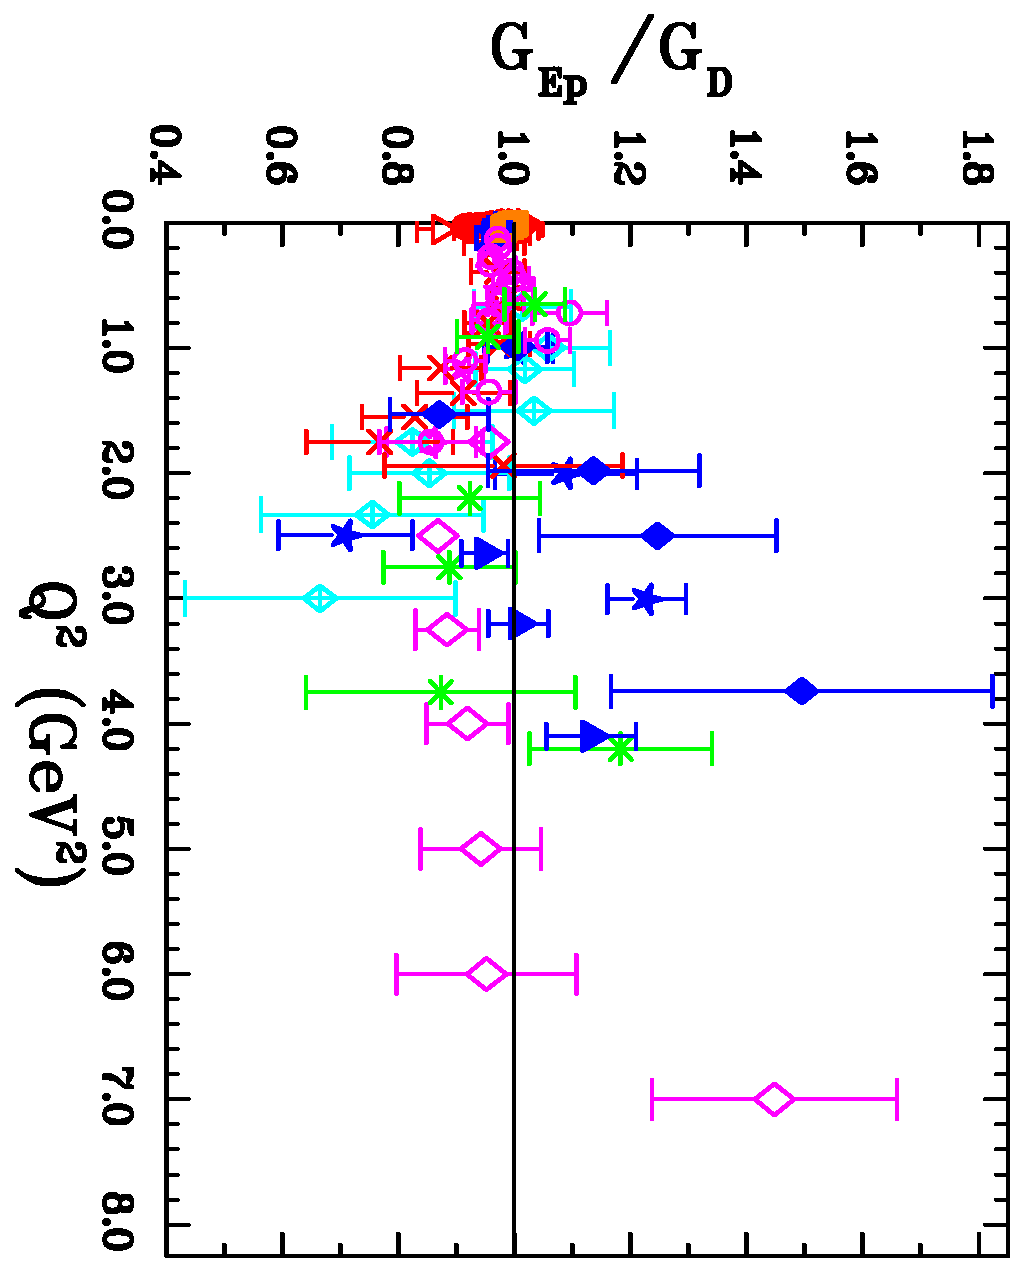
\includegraphics[angle=90]{gepgd_col_lininx.eps}
}
\caption{Ratio $G_{Ep}G_{Mp}$ from all Rosenbluth experiments on a linear scale in $Q^2$; to be compared with the same data displayed on a log scale.}
\label{fig:gepgd_lin}
\end{center}
\end{figure}

The modern version of the Rosenbluth separation technique takes advantage 
of the linear dependence in $\epsilon$, in the reduced 
cross section $\sigma_{red}$, based on Eq. (\ref{eq:csgegm}), as follows:
\begin{eqnarray}
\left(\frac{d\sigma}{d\Omega}\right)_{red} &=& \epsilon(1+\tau)\frac{E_{beam}}{E_e}\left(\frac{d\sigma}{d\Omega}\right)_{exp} / \left(\frac{d\sigma}{d\Omega}\right)_{Mott} \nonumber \\
&=& \tau G_{M}^2+\epsilon G_{E}^2,
\label{eq:redcs}
\end{eqnarray}
\noindent showing that the reduced cross section $\sigma_{red}$ is expected to have a linear dependence on $\epsilon$, with slope proportional 
to $G_{E}^2$ and intercept equal to $\tau G_{M}^2$. To illustrate the method, the reduced cross section data, $\sigma_{red}$, of ref. 
\cite{qattan05} are shown in Fig. \ref{fig:geplt1}. The 
corresponding form factor ratios are shown in Fig. \ref{fig:gepgd_cs} on a background of other form factor ratios obtained from Rosenbluth
separations. Also shown on this figure are the results of the first two recoil polarization experiments obtained in hall A, triangle symbols. 
\cite{jones,punjabi05A,punjabi05B,gayou:2002}. The dichotomy between cross section (Rosenbluth separation) and recoil polarization results is very obvious indeed from this figure.

\subsubsection{Proton Radius}

In a general sense the elastic {\it {ep}}  cross section is related to the Mott cross section for a spin $\frac{1}{2}$ electron
without internal structure times the Fourier transform of the charge and/or magnetization density of the target nucleon as follows:
\begin{equation}
\sigma(\theta_e)=\sigma_{Mott}\times\left|\int_{volume}\rho(\vec r)exp{i\vec{q}.\vec r}d^3\vec r\right|^2
\end{equation}    
\noindent where $\rho(\vec r)$ is either the electric- or the magnetic spacial distribution function. If follows, for the particular of 
the electric form factor G$_{Ep}(Q^2)$, that for short distances it can be expanded in terms of even moments of the distance $<r_e^{2n}>$ as:
\begin{equation}
G_{Ep}=1 - \frac{1}{6}{Q^2<r_e{^2}>} + \frac{1}{120}{Q^4<r_e{^4}>} ... 
\label{eq:rms}
\end{equation}
\noindent Hence for very small distance within the nucleon, the mean-square radius of the proton can be obtained from the derivative of
 Eq. \ref{eq:rms} 
\begin{equation}
\frac{dG_{Ep}}{dQ^2}=-\frac{1}{6}|left{r_e{^2}}|right_{at Q^2=0}
\end{equation}
\noindent from which follows the relation 
\begin{equation}
<r_e{^2}> = - 6|left\frac{dG_{Ep}}{dQ^2}|right_{at Q^2=0}; 
\end{equation}
A similar relation holds for the magnetic radius $<r_m{^2}>$.
Many electron scattering experiments have obtained values of $<r_e{^2}>$ by fitting low Q$^2$ cross section data \cite{sick:2003,sick:2014} ; 
$<r_m{^2}>$ is more difficult to obtain as its contribution to the cross section is weighted down by the factor $\tau$ (see Equ. \ref{eq:csgegm}). 

The proton radius can also be obtained from precise measurements of the Lamb shift energies either in the hydrogen atom 
(Ref. \cite{melnikov:2000}), or in muonic hydrogen (Ref. \cite{antognini:2013}). 
In both cases the 2S-2P Lamb shift is affected by the fact that the S-state wave function is maximum at the hydrogen's center,
 while the P-state has minimal overlap with the hydrogen nucleus. Recent measurements of the muonic Lamb shift energies at PSI have produced
values of $<r_e{^2}>$ which are smaller than the mean value of all electron scattering experiments by 7 $\sigma$ (\cite{pohl:2013}).  


\subsection{Formalism of double polarization experiments}

In 1968 and 1974 Akhiezer and Rekalo \cite{akh1A,akh1B} discussed the interest of measuring 
an interference term of the form  $G_{E}G_{M}$ by measuring the transverse 
component of the recoiling proton polarization in $\vec e p~\rightarrow~e \vec p$  
at large Q$^2$, to obtain $G_E$ in the presence of a dominating $G_M$.
In a review paper Dombey \cite{dombey} emphasized the virtues of measurements with a polarized lepton beam 
on a polarized target to obtain polarization observables. 
Also much later in 1982 Arnold, Carlson and Gross \cite{arnold} discussed in detail, that the best way 
to measure the neutron and proton form factors would be to use the $^2H( \vec e,e' \vec n)n$ 
and $^1H( \vec e,e' \vec p)$ reactions, respectively.

Indeed, both the recoil polarization and target asymmetry measurement methods have
been used successfully to measure the proton and neutron form factors to high 
four momentum transfer, $Q^2$, at Jefferson Lab. These methods have been used also at MIT-Bates, the Mainz 
Microtron (MAMI),and Nationaal Instituut voor Kernfysica en Hoge Energie Fysica (NIKHEF), to make precise 
proton and neutron form factor measurements at lower $Q^2$. Both methods are discussed below, with 
benefits and drawbacks of using polarized target and focal plane polarimeter.  


\subsubsection{Recoil polarization method}

\label{subsubsec:poltrans}

With a longitudinally polarized electron beam and an un-polarized hydrogen target, the 
polarization of the incoming electron is transferred to the proton via an exchange of a virtual photon as 
shown in Fig. \ref{fig:nlt}. 
For elastic ep 
scattering with a longitudinally polarized electron beam, the only non-zero
polarization transfer observables are the longitudinal and transverse
polarizations, $P_{\ell}$ and $P_t$. For single photon exchange, the 
transferred polarization can be written in terms of the Sachs form factors as:

\begin{eqnarray}
I_o P_n & = & 0  \nonumber \\
%I_oP_t & = & -hP_e2 \sqrt{\tau(1+\tau)}\tan\frac{\theta_e}{2} G_EG_M  \nonumber \\ 
I_oP_\ell & = & hP_e\frac{(E_{beam}+E_{e})}{M}\sqrt{\tau(1+\tau)}\tan^2\frac{\theta_e}{2}  G_M^2 \nonumber \\ 
I_oP_t & = & -hP_e2 \sqrt{\tau(1+\tau)}\tan\frac{\theta_e}{2} G_EG_M 
\end{eqnarray}

\noindent
where $h = \pm 1$ and $P_e$ are the beam helicity and polarization, respectively; $E_{beam}$ and $E_{e}$ are the incident and scattered 
electron energies, $\theta_{e}$ is the electron scattering angle, and M is the 
mass of the proton; $I_o=G_E^2+\frac{\tau}{\epsilon}G_M^2$, is the unpolarized cross section and 
$\epsilon=[1+2(1+\tau)\tan^2\frac{\theta_{e}}{2}]^{-1}$ is the longitudinal polarization of the virtual photon.


%%%%%%%%%%%%%%Figure 5 kinematics
\begin{figure}
\begin{center}
\resizebox{0.45\textwidth}{!}{%
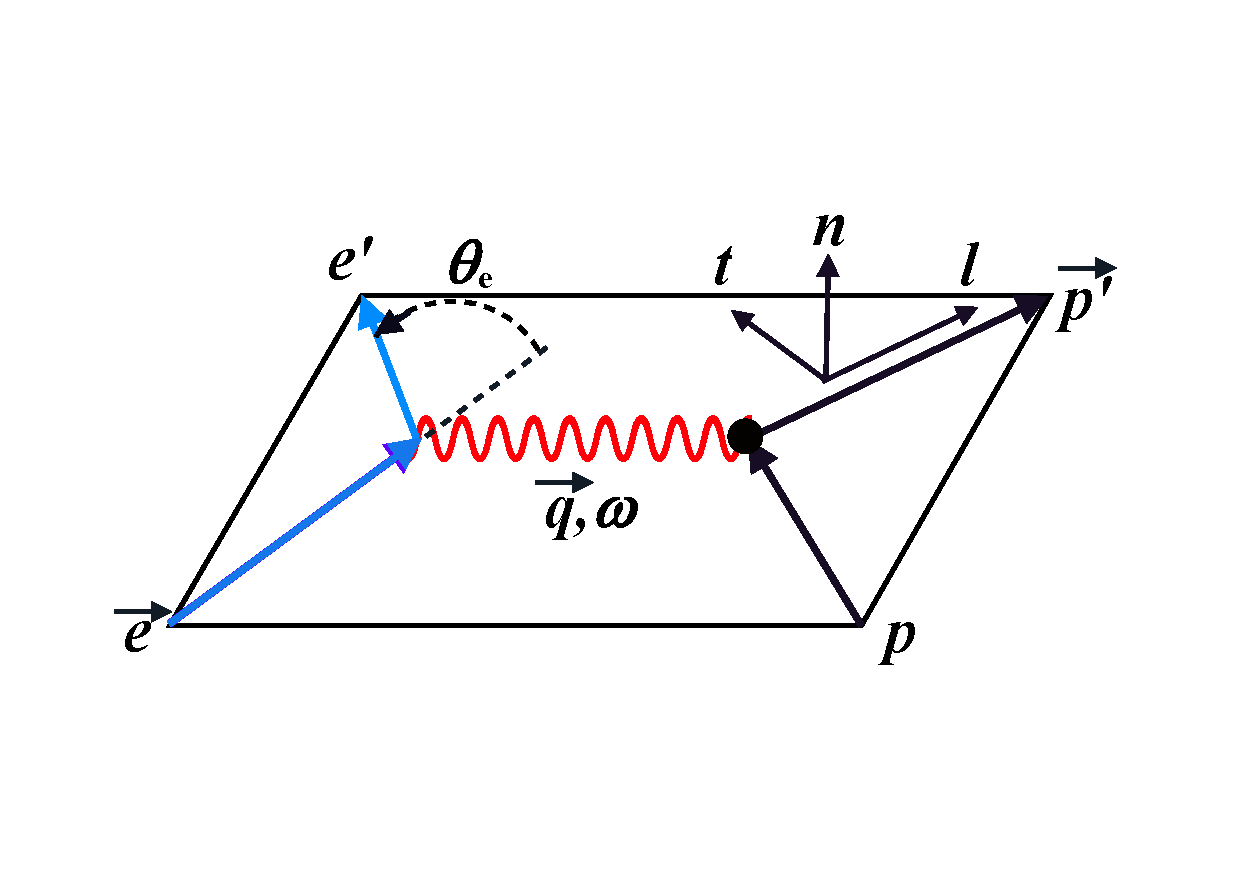
\includegraphics{ep_recoilpol_10312014.pdf}
}
\caption{Illustration of the kinematics and polarization of the recoil proton for $\vec e p\rightarrow e' \vec p$.}
\label{fig:nlt}
\end{center}
\end{figure}

The ratio of $G_E$ and $G_M$ is then directly obtained from the ratio of the two polarizations $P_t$ and $P_{\ell}$
components:
\begin{equation}
\frac{G_{E}}{G_{M}}=-\frac{P_{t}}{P_{\ell}}\frac{(E_{beam}+E_{e})} 
{2M}\tan (\frac{\theta_{e}}{2}).
\label{eq:ratio}
\end{equation}

In the one-photon exchange process, the form factors depend only on $Q^2$ and a deviation from constant would 
indicate a mechanism beyond the Born approximation. For each $Q^2$, a single measurement of the azimuthal angular
distribution of the proton scattered in a secondary target gives both the longitudinal and transverse polarizations.
Thus the ratio of electric to magnetic form factors of the proton is obtained directly from a simultaneous 
measurement of the two recoil polarization components. The knowledge of the beam polarization and of the analyzing power of the 
polarimeter is not needed to extract the ratio, $G_{E}/G_{M}$.  The kinematic factors in Eq. (\ref{eq:ratio}) are
typically known to a precision far greater than the statistical precision of the recoil polarization components.



\subsubsection{Asymmetry with polarized targets}
\label{subsubsec:Asymmetry}


It was discussed by Dombey \cite{dombey} in a review paper in 1969 that the nucleon form factors 
can be extracted from the scattering of longitudinally polarized electrons off
a polarized nucleon target. 
In the one photon exchange approximation, the elastic electron nucleon
scattering cross section can be written reaction en as a sum of two parts: $\Sigma$, which corresponds to
the unpolarized elastic differential cross section $d\sigma/d\Omega_e$, and a polarized part $\Delta$, which is
non-zero only if the electron beam is longitudinal polarized \cite{donnelly,raskin};

\begin{equation} 
\sigma_{h} = \Sigma + h \Delta, \\
\label{eq:asymm}
\end{equation}
\noindent
where h is the beam helicity, and $\Sigma$ the unpolarized elastic {\it {ep}} cross section can be written as:
\begin{equation} 
\Sigma =  \left(\frac{d\sigma}{d\Omega}\right)_{Mott}{\frac{E_e}{E_{beam}}}{\frac{1}{1+\tau}}\left[G_E^2 + \frac{\tau}{\epsilon}G_M^2 \right]. \\
\label{eq:Sigma}
\end{equation}

The polarized part of the cross section, $\Delta$, with two terms related to the directions of the target polarization, 
$\vec{P}(\theta^{\ast} \phi^{\ast})$, is given by \cite{donnelly,raskin}: 
\begin{eqnarray}
\Delta & = & -2 \left(\frac{d\sigma}{d\Omega}\right)_{Mott} \frac{E_e}{E_{beam}}\tan\frac{\theta_e}{2} \sqrt{\frac{\tau}{1+\tau}} \nonumber \\
& & \Big(\sqrt{\tau\big[1+(1+\tau)\tan^2\frac{\theta_e}{2}\big]} \cos\theta^{\ast}G_M^2  \nonumber \\
&+&\sin\theta^{\ast}\cos\phi^{\ast}G_E G_M  \Big)
\label{eq:delta}
\end{eqnarray}
\noindent
where $\theta^{\ast}$ and $\phi^{\ast}$ are the polar and 
azimuthal laboratory angles of the target polarization vector with $\vec q$ in the $\vec z$
direction and $\vec y$ normal to the electron scattering plane, as shown 
in Figure \ref{fig:epkin_asym}.

%%%%%%%%%%%%%Fig 6 kinematics
\begin{figure}
\begin{center}
\resizebox{0.45\textwidth}{!}{%
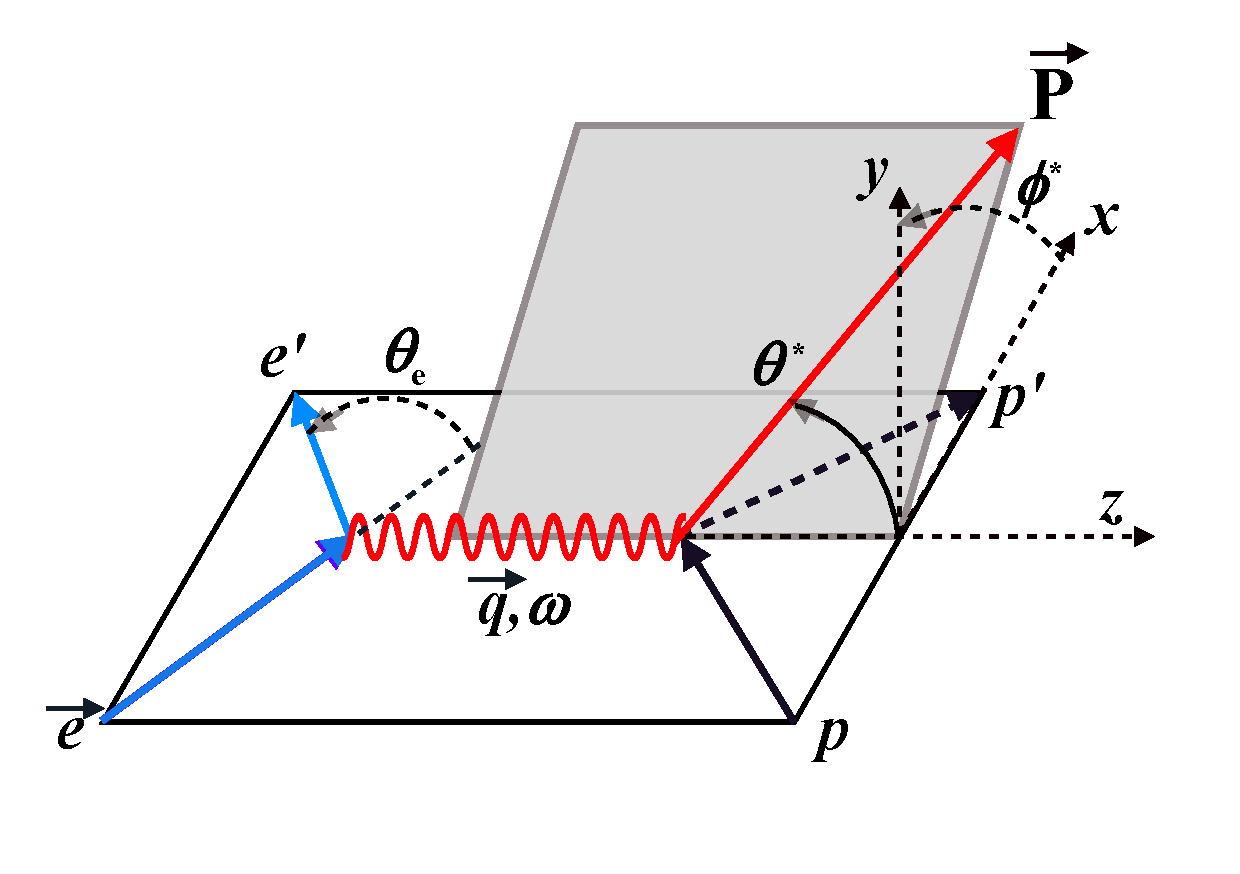
\includegraphics{ep_asymmetry_10312014.pdf}
}
\caption{Illustration of the kinematics and orientation of the target polarization $\vec P$, for the reaction $\vec e \vec n \rightarrow e' n$. }
\label{fig:epkin_asym}
\end{center}
\end{figure}

The physical asymmetry $A$ is then defined as 
\begin{equation}
A=\frac{\sigma_{+} -\sigma_{-}}{\sigma_{+} + \sigma_{-}}=\frac{\Delta}{\Sigma},
\label{eq:asy}
\end{equation}
\noindent
where $\sigma_+$ and $\sigma_-$ are the cross sections for the two beam helicities. 

For a longitudinally polarized beam and polarized target, the measured asymmetry, $A_{meas}$, is 
related to the physical asymmetry, $A$, by 
\begin{equation}
A_{meas}=P_{beam}P_{target}A,
\label{eq:asy1}
\end{equation}
\noindent
where $P_{beam}$ and $P_{target}$ are electron beam and target polarization, respectively, and 
 $A$ can be obtained using Eqs. (\ref{eq:Sigma}) and (\ref{eq:delta}),  
\begin{eqnarray}
A &=&-\frac{2\sqrt{\tau(1+\tau)}\tan\frac{\theta_e}{2}}{G_E^2+\frac{\tau}{\epsilon}G_M^2}
\Big[ \sin\theta^{\ast}\cos\phi^{\ast}G_E G_M \nonumber \\
&+& \sqrt{\tau\big[1+(1+\tau)\tan^2\frac{\theta_e}{2}\big]} \cos\theta^{\ast}G_M^2 \Big].
\label{eq:asy2}
\end{eqnarray}

From Eq. (\ref{eq:asy2}), it is apparent that to extract $G_{E}$, the target polarization 
in the laboratory frame must be perpendicular with respect to the momentum transfer vector ${\vec q}$
and within the reaction plane, with $\theta^{\ast}= \pi/2$ and $\phi^{\ast}= 0^o$ or $180^o$. 
For these conditions, the physical asymmetry $A$ in Eq. (\ref{eq:asy2}) simplifies to:
\begin{equation}
A_{perp}=\frac{-2\sqrt{\tau(1+\tau)}\tan\frac{\theta_e}{2} \frac{G_E}{G_M}}{(\frac{G_E}{G_M})^2+\frac{\tau}{\epsilon}}.
\label{eq:asy3}
\end{equation}
\noindent
As $(G_E/G_M)^2$ is quite small, $A_{perp}$ is approximately proportional to $G_E/G_M$. In practice, the second term in 
Eq. (\ref{eq:asy2}) is not strictly zero due to the finite acceptance of the detectors, but these effects are small and depend
on kinematics only in first order and can be corrected for, so the ratio $G_E/G_M$ is not affected directly.

The discussion above is only applicable to a free electron-nucleon scattering. 
For a quasi-elastic electron scattering from a nuclear targets, like $^2$H or $^3$He, corrections are required for several nuclear effects. 

\subsection{Two-photon exchange}

In the one-photon exchange process, the form factors depend only on $Q^2$
and a deviation from constant would indicate a mechanism beyond
the Born approximation. 

In the general case, 
elastic $ep$ scattering can be described by three
complex amplitudes \cite{diehl:2013,guichon}:  $\tilde{G}_M$, $\tilde{G}_E$,
and $\tilde{F}_3$, the first two 
chosen as generalizations of the Sachs 
electric and magnetic form factors, $G_E$ and $G_M$, and the 
last one, $\tilde{F}_3$, vanishing in case of Born approximation.
The reduced cross section, $\sigma _{red}$, and the
proton polarization transfer components $P_t$ and $P_l$,
including two-photon exchange formalism, can be written as \cite{guichon}:

\begin{eqnarray}
\frac{\sigma _{red}}{G_M^2}&=& 1+\frac{\varepsilon R^2}{\tau }+2\frac{\Re\delta \tilde{G}_M}{G_M} \nonumber \\
&+& 2R\varepsilon \frac{\Re\delta \tilde{G}_E}{\tau G_M}+ 2\left(1+\frac{R}{\tau }\right){ \varepsilon Y_{2\gamma }}
\label{eq:siggen}
\\
P_t&=&-\sqrt{\frac{2\varepsilon(1-\varepsilon)}{\tau}}
\frac{G_M^2}{\sigma _{red}}  \nonumber \\
& &\left(R+
R\frac{ \Re\delta \tilde{G}_M}{G_M}
+\frac{ \Re\delta \tilde{G}_E}{G_M}
+{ Y_{2\gamma }}\right)
\label{eq:ptgen}
\\
P_l&=&\sqrt{(1-\varepsilon ^2)}\frac{G_M^2}{\sigma _{red}} \nonumber \\
& &\left(1+2\frac{ \Re\delta \tilde{G}_M}{G_M}+\frac{2}{1+\varepsilon }{ \varepsilon Y_{2\gamma }}\right)  %\vspace{0.25in}
\label{eq:plgen}
\mbox{,}
\end{eqnarray}
where:
\begin{eqnarray}
\Re\tilde{G_M}(Q^2,\varepsilon)&=&G_M(Q^2)+\Re\delta \tilde{G_M}(Q^2,\varepsilon)  \\ %\vspace{0.25in}
\label{eq:regm}
\Re\tilde{G_E}(Q^2,\varepsilon)&=&G_E(Q^2)+\Re\delta \tilde{G_E}(Q^2, \varepsilon) 
\label{eq:rege} \\  %\vspace{0.25in}
R(Q^2)&=&G_E(Q^2)/G_M(Q^2) \nonumber 
\end{eqnarray}

Here $\tau=Q^{2}/4M_{p}^{2}$, 
and $\varepsilon =[1+2(1+\tau)\tan^2\frac{\theta_e}{2}]^{-1}$,
where  $\theta_e$ is the lab electron scattering angle.
While the Sachs form factors depend only on $Q^2$, in the general case the
amplitudes depend also on $\varepsilon$.
%The $Y_{2\gamma}$ function defined above is
%related to the third amplitude $\tilde{F}_3$. 
The  reduced cross section
and the transferred proton polarization components are sensitive only to the real part
of the amplitudes. 

In Born approximation only the first term remains in the reduced cross 
section, $\sigma _{red}$, and the
proton polarization transfer components $P_t$ and $P_l$ are :
\begin{eqnarray}
{\sigma _{red}}/{G_M^2}&=&
1+\frac{\varepsilon R^2}{\tau }
\label{eq:sigborn}
\\
P_t&=&-\sqrt{\frac{2\varepsilon(1-\varepsilon)}{\tau}}
\frac{G_M^2R}{\sigma _{red}}
\label{eq:ptborn}
\mbox{,}  \\
%\; \; \;
P_l&=&\sqrt{(1-\varepsilon ^2)}
\frac{G_M^2}{\sigma _{red}}
\label{eq:pborn}
%\label{eq:plborn}
\end{eqnarray}

\section{Recent developments; to be relocated}

The experimental and theoretical situation for the nucleon form factors were reviewed extensively in the 7 years following
publication of the results of the first recoil polarization experiment at Jefferson Lab \cite{jones}. Chronologically
these reviews include Gao \cite{gaoA,gaoB}, Hyde-Wright et al. \cite{charleskees}, Perdrisat et al. \cite{perdrisat:2006} and 
Arrington et al. \cite{arrreview}, Arrington et al \cite{arrington:2011}, Cloet et al. \cite{cloet:2008}
and Perdrisat and Punjabi \cite{scholar}. At this point in time, the double-polarization method had been used up to 5.6 GeV$^2$
for the proton form factor ratio $G_{Ep}/G_{Mp}$ (\cite{jones,punjabi05A,punjabi05B,gayou:2001}, and 1.45 GeV$^2$ for $G_{En}/G_{Mn}$. 
Recent polarization experiments at JLab for $G_{Mn}$ to a Q$^2$ of 0.6 GeV$^2$ \cite{anderson} had been published, and a 
mix of polarization and cross section had been obtained up to 5 GeV$^2$ for $G_{Mn}$, the latest  using the cross section
ratio method, to obtain $G_{Mn}$ from the measured 
${\frac{\frac{d\sigma}{d\Omega}[^2H(e,e'n)_{QE}]}{\frac{d\sigma}{d\Omega}[^2H(e,e'p)_{QE}]}}$ ratio \cite{brooksA,brooksB}.

The principal revelation coming out of the first $G_{Ep}/G_{Mp}$ experiment using recoil polarization was the systematic
decrease of this ratio with increasing Q$^2$. There existed data from the 1970's which suggested a similar behavior, 
although they were limited to Q$^2$ smaller than 3 GeV$^2$, and had large uncertainties. Interestingly, at that time, 
models based on vector meson dominance (VMD) \cite{hohler,gariA,gariB} were predicting a rapid decrease of the ratio
 $G_{Ep}/G_D$, reaching a value of 0.5 at Q$^2$ of 4 GeV/c. In the same period, a first paper from the Stanford group
\cite{litt} suggested a drastically different Q$^2$ dependence of the same ratio, $G_{Ep}/G_{Mp}$, with values reaching
1.35+/-0.3 at Q$^2$=3.6 GeV$^2$ (verify these numbers). The complete set of experimental results derived from cross 
section measurements is shown in Fig. \ref{fig:gepgd_cs} and \ref{fig:gmpgd_cs}. It includes the most recent JLab results
 of \cite{christy,qattan05}.

%%%%%%%%%%%%%%%%%%%%%%%%%%Figure 7
\begin{figure}
\begin{center}
\resizebox{0.45\textwidth}{!}{%
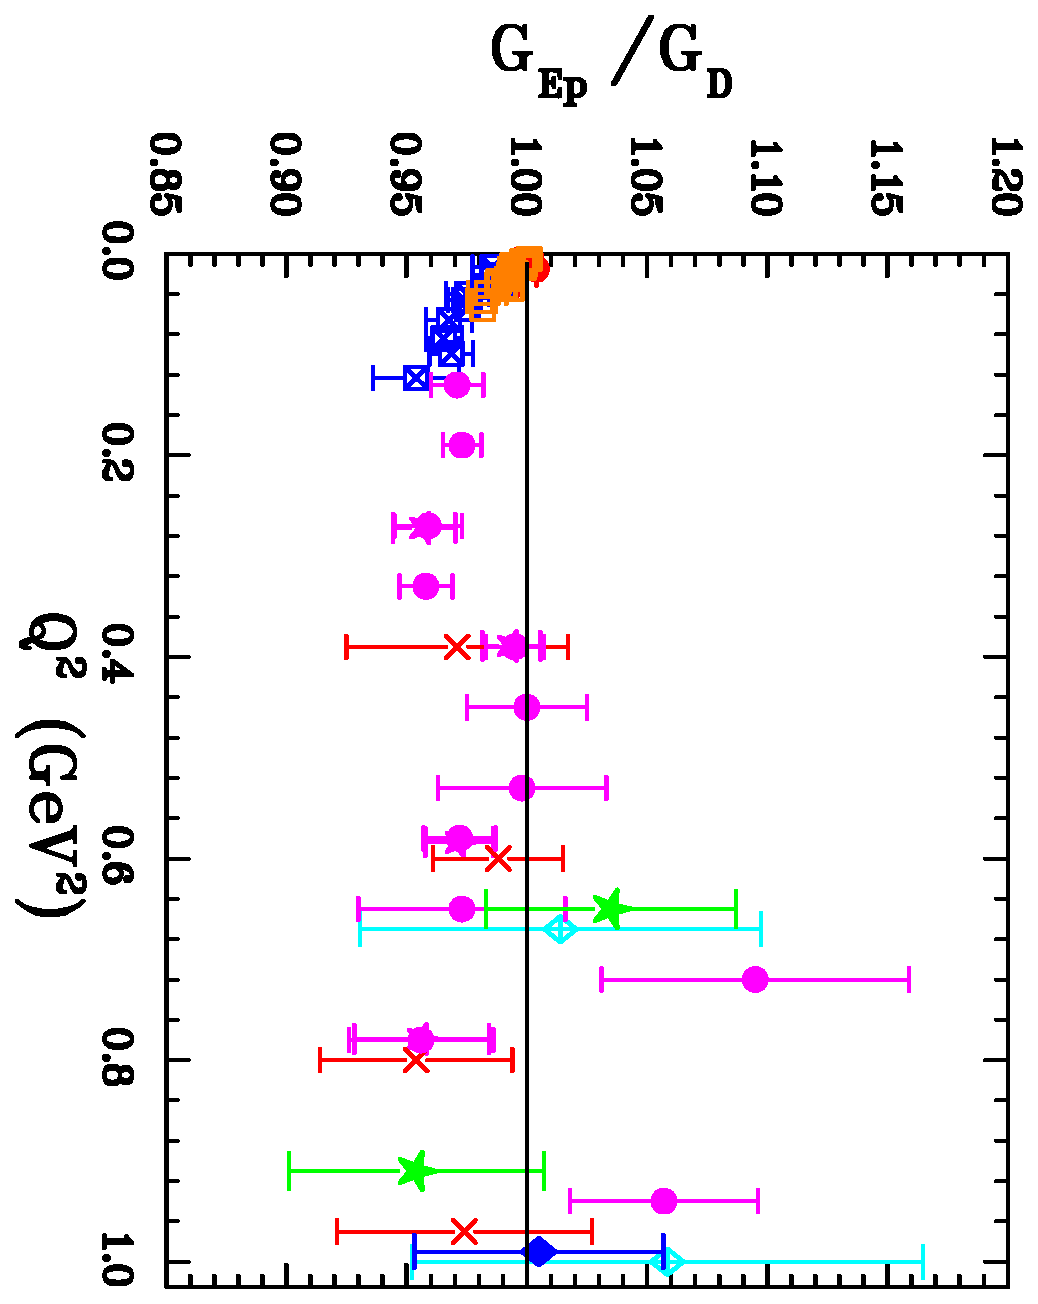
\includegraphics[angle=90]{gepgd_col_lininx_xmax1.eps}
}
\caption{Low $Q^2$ behavior of the $G_{Rp}/G_D$ ratio for Q$^2$ smaller than 1 GeV$^2$ for Rosenbluth data, illustrating the very small deviation from a constant of this ratio for small $Q^2$.}
\label{fig:gepgd}
\end{center}
\end{figure}

%%%%%%%%%%%%%%%%%% Figure 8
\begin{figure}
\begin{center}
\resizebox{0.45\textwidth}{!}{%
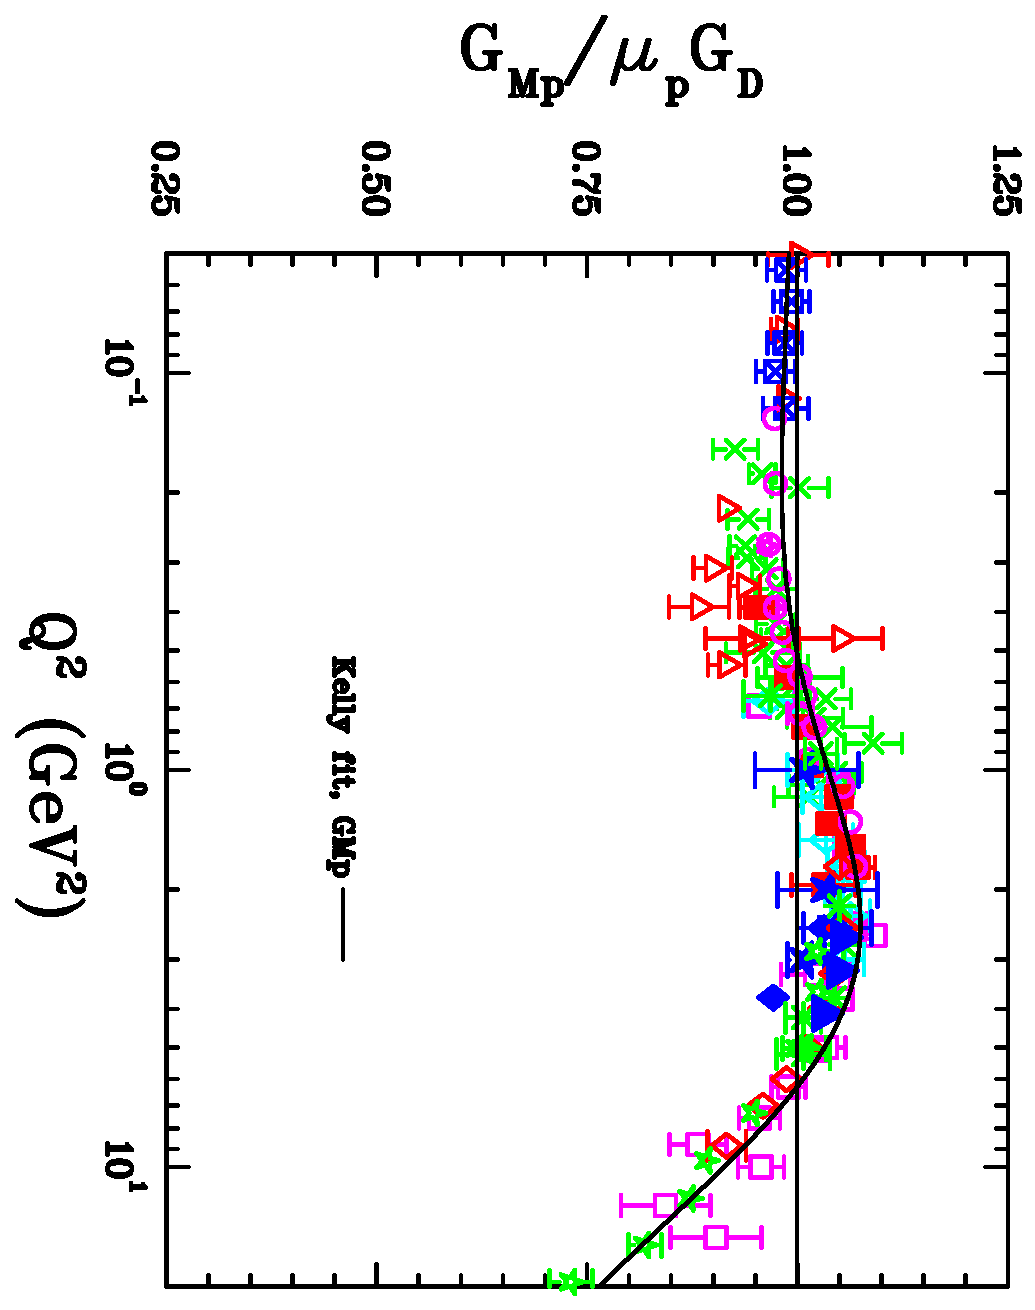
\includegraphics[angle=90]{gmpgd_spS.eps}
}
\caption{Rosenbluth values of $G_{Mp}/\mu_pG_D$ including all published data, for comparison with Fig. \ref{fig:geplt1}.} 
\label{fig:gmpgd_cs}
\end{center}
\end{figure} 

Since the last review paper was published, considerable theoretical work was performed. Some of the original models
discussed in the 1970's, in particular the original Vector Dominance (VMD), as well as the Constituent Quark
(CQM) models were revisited, made relativistic, then more of less left the front row, with the exception of 
Lomon \cite{lomon}, Bijker \cite{bijker} and others.

The proton form factors were originally introduced in non-relativistic scattering, as the three-dimensional Fourier
transform of the charge density \cite{hofs53,wilsonrr}. However the proton recoil implies that the electron
 is interacting with a moving charge distribution. Already for Q$^2$=0.25 GeV$^2$, the recoil proton relativistic 
boost factor $\gamma$ is 1.1, corresponding to $v/c=0.41$.
The argument that form factors are Fourier transforms of nucleon density in the Breit frame was abandoned, as this 
frame's velocity in the Lab frame is different for every Q$^2$.

The proton in its ground state is not necessarily spherically symmetric, but can show a typical multipole shape, 
when referred to the spin direction of one of its quarks (constituents) relative to the nucleon spin orientation
 \cite{miller:2003}. %shape of the proton

The wave front or infinite momentum frame densities are invariant, two-dimensional transverse charge and magnetization distribution, 
and are drastically different
from the non-relativistic ones \cite{miller:2003,carlson:2007}. % transverse densities in imf

Elastic ep scattering in the 1 to 10 GeV$^2$ range of 4-momentum squared transfer is
the domain of non-perturbative quantum chromodynamics (QCD); as a consequence of Dynamical Chiral Symmetry
Breaking, valence quarks acquire a mass of order $M_p/3$ in the infrared limit. \cite{cloet:2008b,cloet:2008}

   Scaling as a consequence of Perturbative QCD may have visible consequences even in the non-perturbative
 domain \cite{Galynskii:2013} 

The di-quark structure of the nucleon has observable consequences \cite{cloet:2012cy}

The mass of the dressed quarks originates from the QCD vacuum; it results
from accretion of quark-antiquark pairs from decaying gluons spontaneously emerging from the vacuum \cite{cloet:2008}. 

Assuming isospin symmetry one can obtain flavor separated dressed quark form
factors from simple linear relations between the Dirac and Pauli form factors.
The dressed up and down quarks have significantly different form factors 
\cite{cloet:2008,cates:2011,rohrmoser:2011,wilson:2011,Cloet:2013gva,qattan:2013}. 

A zero crossing of GEp, if and when observed,  would provide information on the dressed-quark mass
function \cite{diehl:2013}.

Nucleon form factors determine the parameters of the valence quark GPDs;
these can be used to obtain corresponding valence quark densities \cite{diehl:2013}.

The available data suggest that the isovector electric form factor (GEp-GEn) has a zero near $Q^2$~ 4.3 GeV$^2$;
this feature can be predicted in lattice calculations, from the connected diagram only. \cite{diehl:2013}.
 
Soft  Collinear Effective Theory (SCET), Kivel and Vanderhaeghen(2013)
for two-photon exchange \cite{kivel:2012}.

\section{GEn; to be relocated}

This in preparation  for the neutron section, in particular fig with $\mu_nG_{En}/G_{Mn}$. Nov. 3/14.

%%%%%%%%%%%%%%%%%%% Figure 9
\begin{figure}
\begin{center}
\resizebox{0.45\textwidth}{!}{%
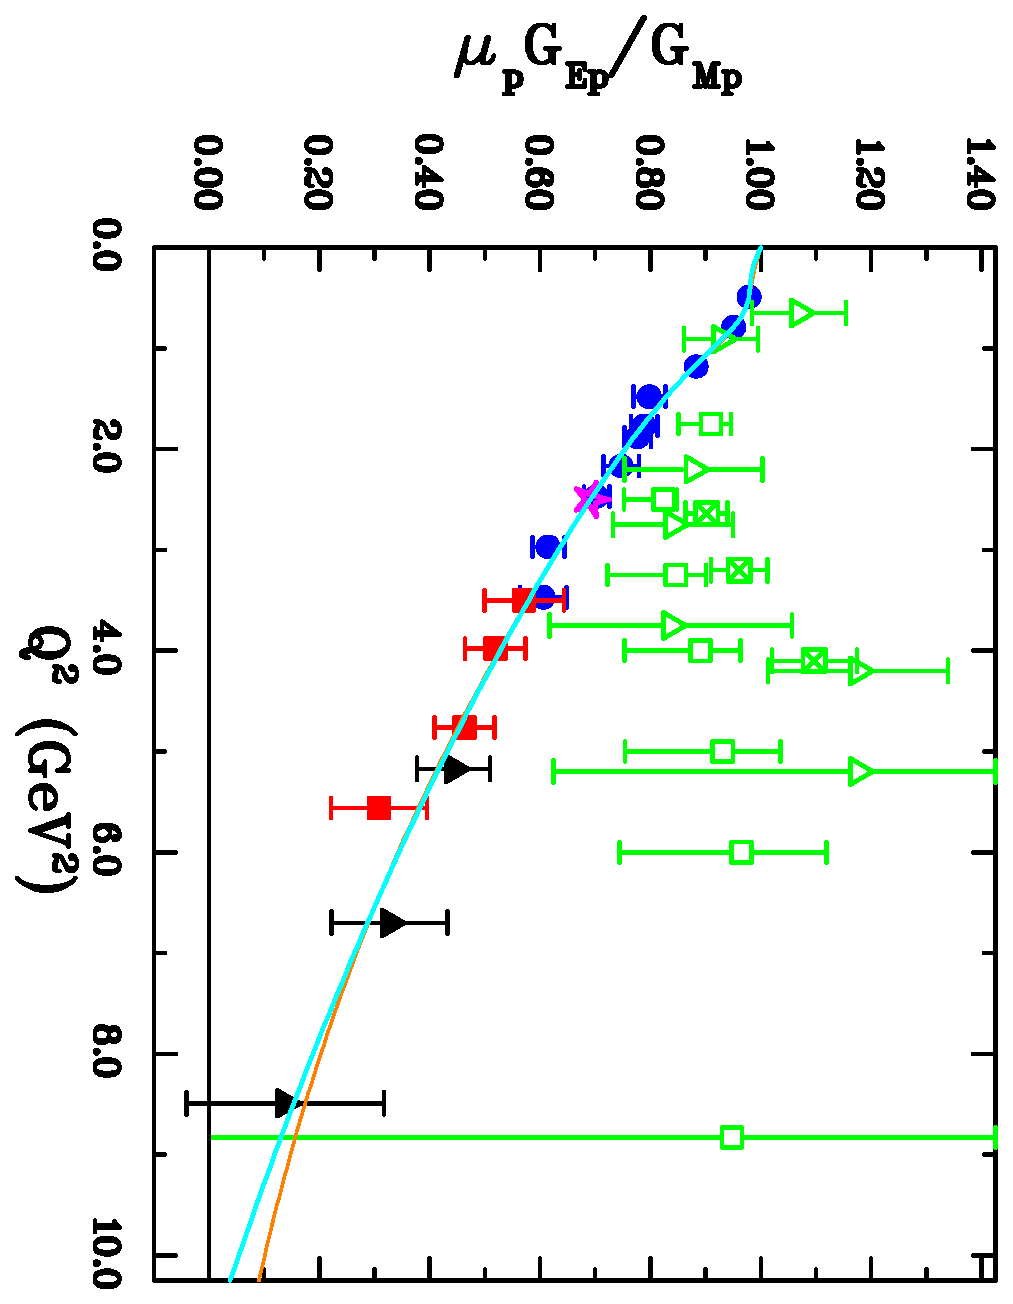
\includegraphics[angle=90]{gepgmp_allpol_allcs_noth_11072014.eps}
}
\caption{All data for the ratio $G_{Ep}/G_{Mp}$ obtained from the three large $Q^2$ recoil polarization experiments at JLab. The dot-dashed curve is a 4 parameter fit without constrain at Q$^2$=0, the solid line is a 7 parameter fit with ratio constrained to 1 at $Q^2$=0; Both fits are of the Kelly type, polynomial over polynomial, with $1/Q^2$ behavior at large Q$^2$.}  
\label{fig:gepgmp}
\end{center}
\end{figure}

%%%%%%%%%%%%%%%%%%%Figure 10
\begin{figure}
\begin{center}
\resizebox{0.45\textwidth}{!}{%
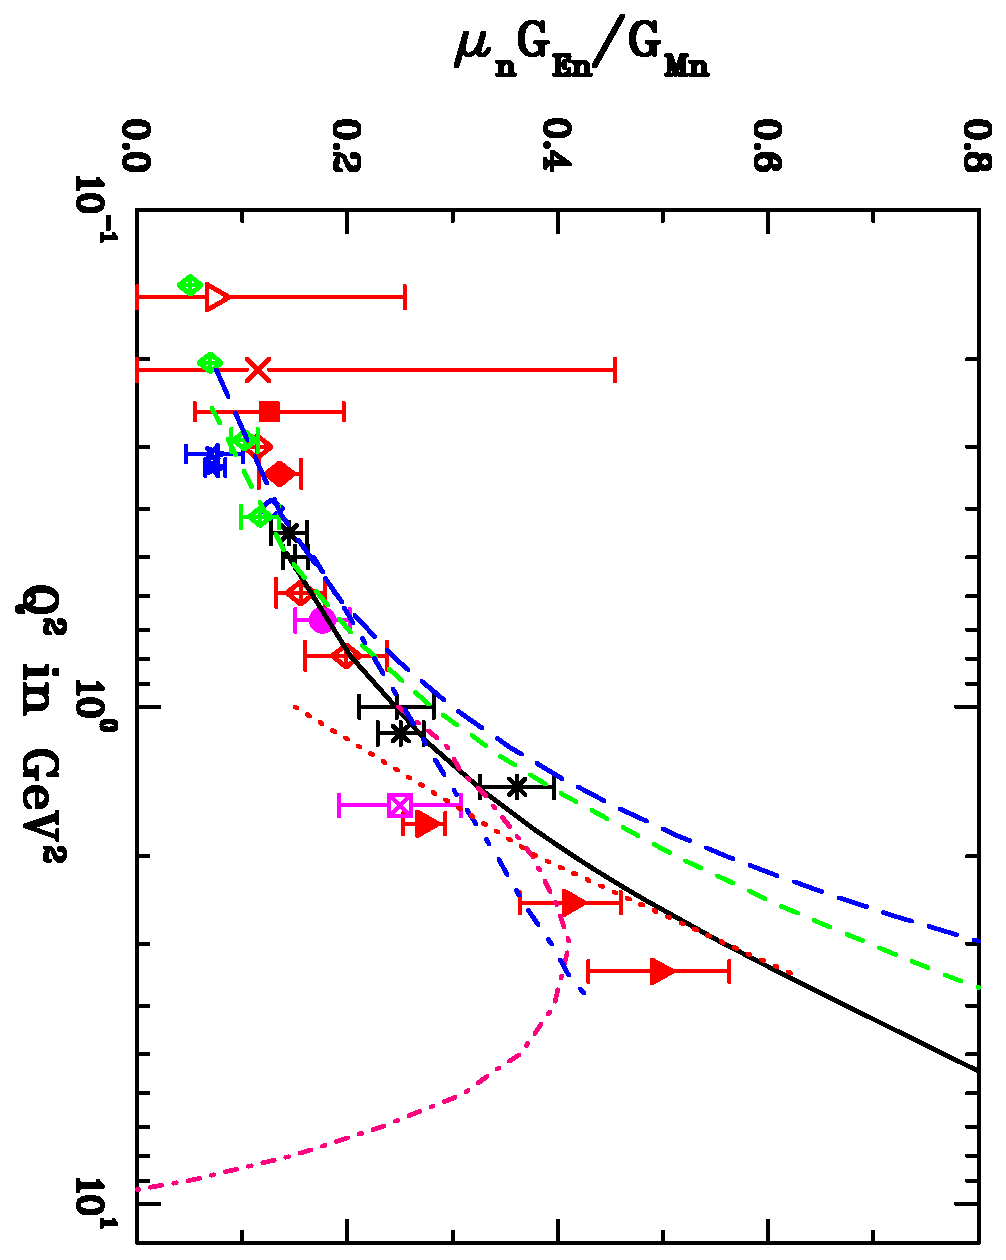
\includegraphics[angle=90]{gengmn_epja_nolbl_10302014.eps}
}
\caption{The complete data base for $G_{En}/G_{Mn}$ from double polarization experiments. Asymmetry with polarized D2 target: \cite{passchier,zhu,warren,geis:2008}, asymmetry with polarized $^3He$ target: \cite{cejones,thompson,meyerhoff:1994,becker,rohe,bermuth,golak:2001,riordan:2010,schlimme:2013}, recoil polarization with D2 target \cite{eden:1994,herberg,ostrick,glazier:2004,madey,plaster}}
\label{fig:neutron2}
\end{center}
\end{figure}

%%%%%%%%%%%%%%%%Figure 11
\begin{figure}
\begin{center}
\resizebox{0.45\textwidth}{!}{%
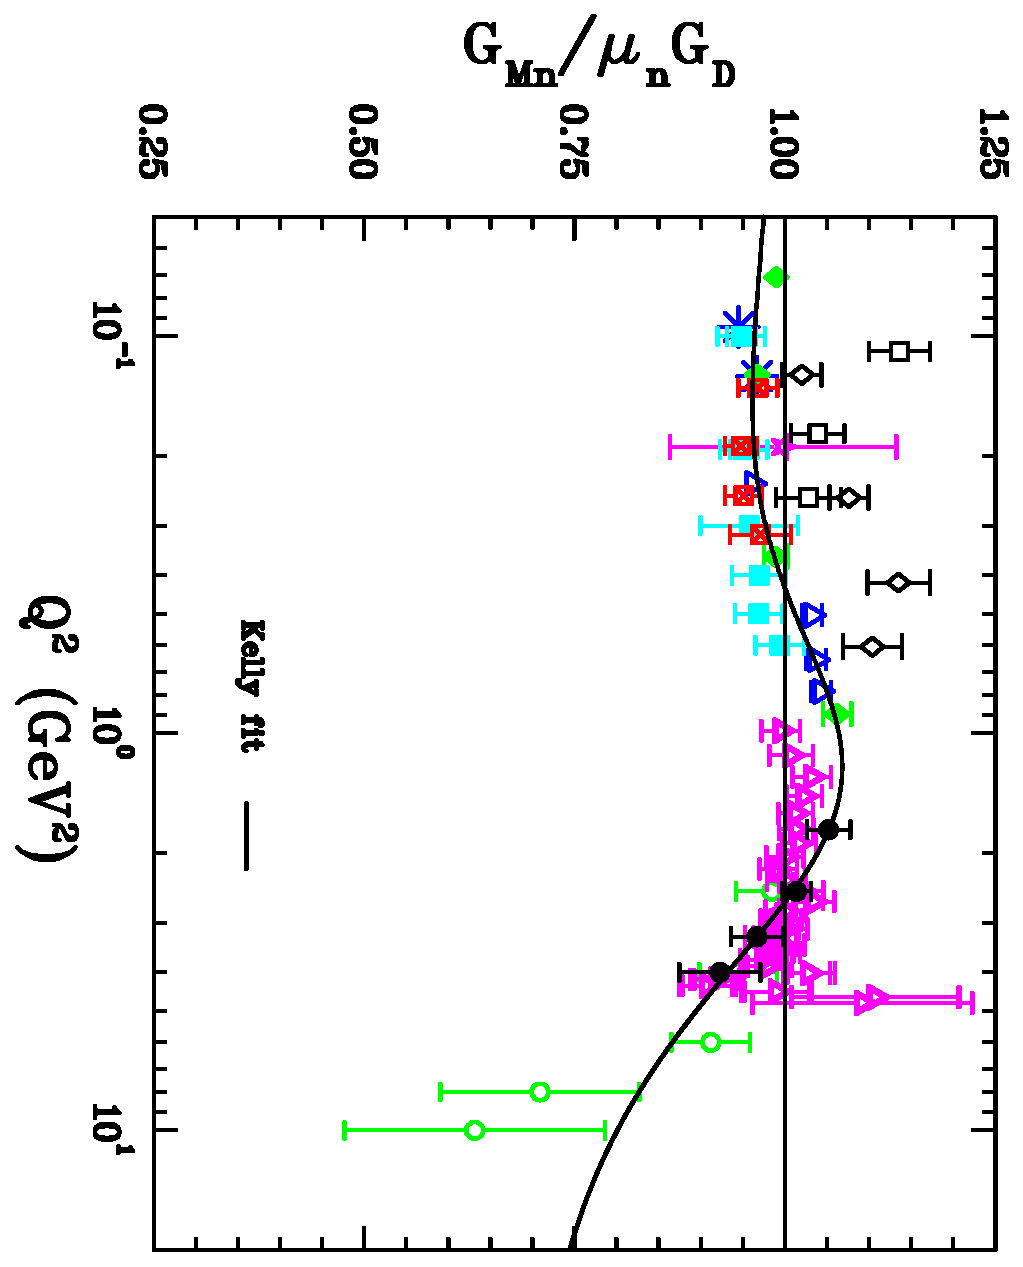
\includegraphics[angle=90.0]{gmngd_log.eps}
}
\caption{The complete data base for $G_{Mn}/\mu_nG_D$. May compare with the equivalent figure for $G_{Mp}/\mu_pG_D$ .}
\label{fig:gmn}
\end{center}
\end{figure}

\section{More Figures}

%%%%%%%%%%%%%%%%%%%%%%%%%%%% Figure 12
\begin{figure}
\begin{center}
\resizebox{0.45\textwidth}{!}{%
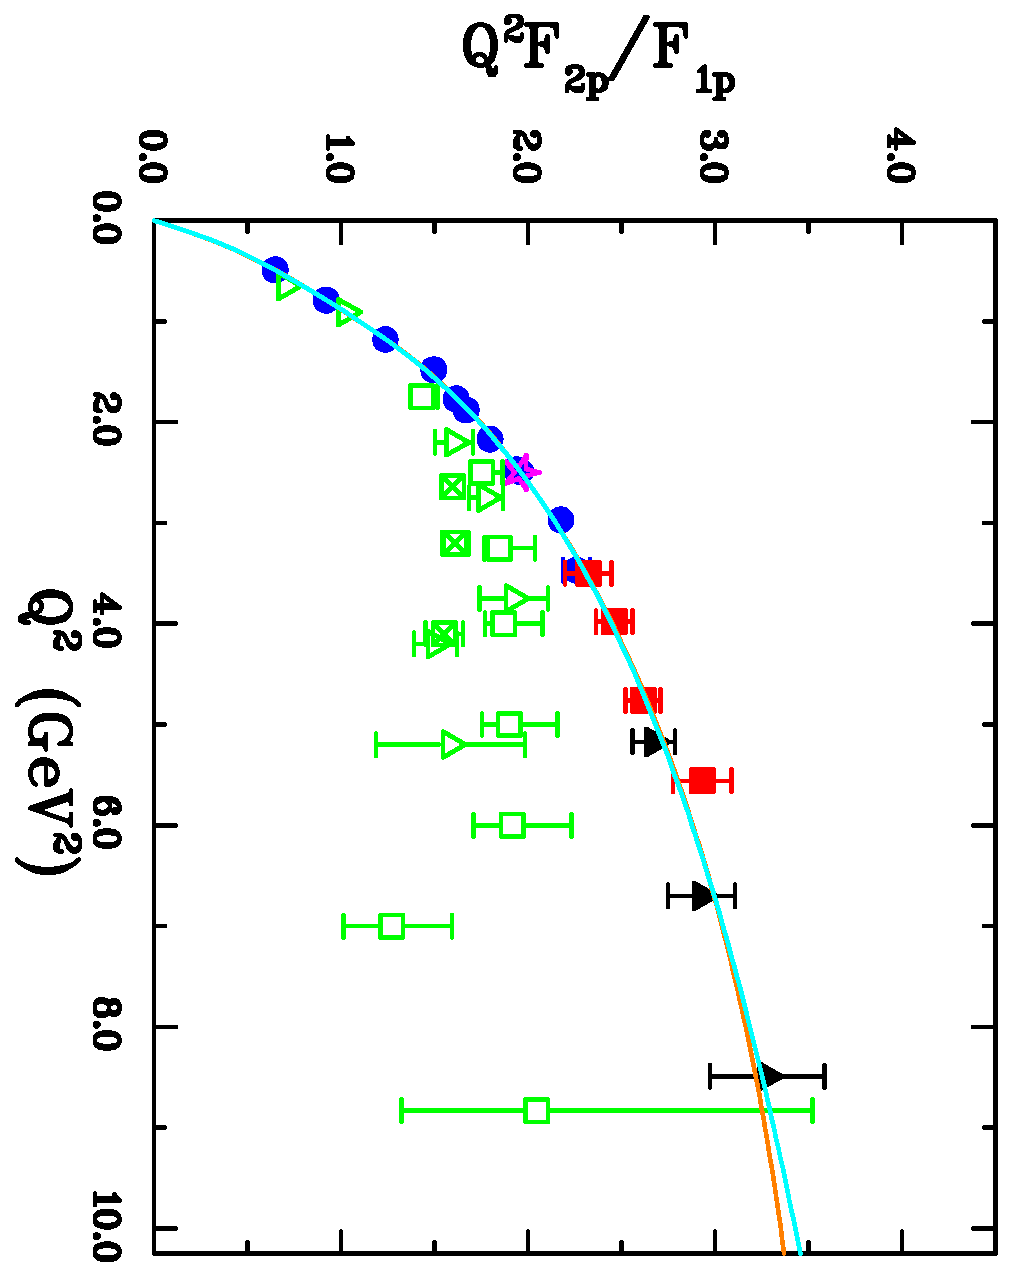
\includegraphics[angle=90]{q2f2f1_allpol_11072014.eps}
}
\caption{Behavior of the ratio $Q^2F_2/F_1$ for the proton, versus $^2$. JLab data for recoil polarization; empty symbols for Rosenbluth data. }.
\label{fig:q2f2f1p}
\end{center}
\end{figure}

%%%%%%%%%%%%%%%%%%%%%%%%%  Figure 13
\begin{figure}
\begin{center}
\resizebox{0.45\textwidth}{!}{%
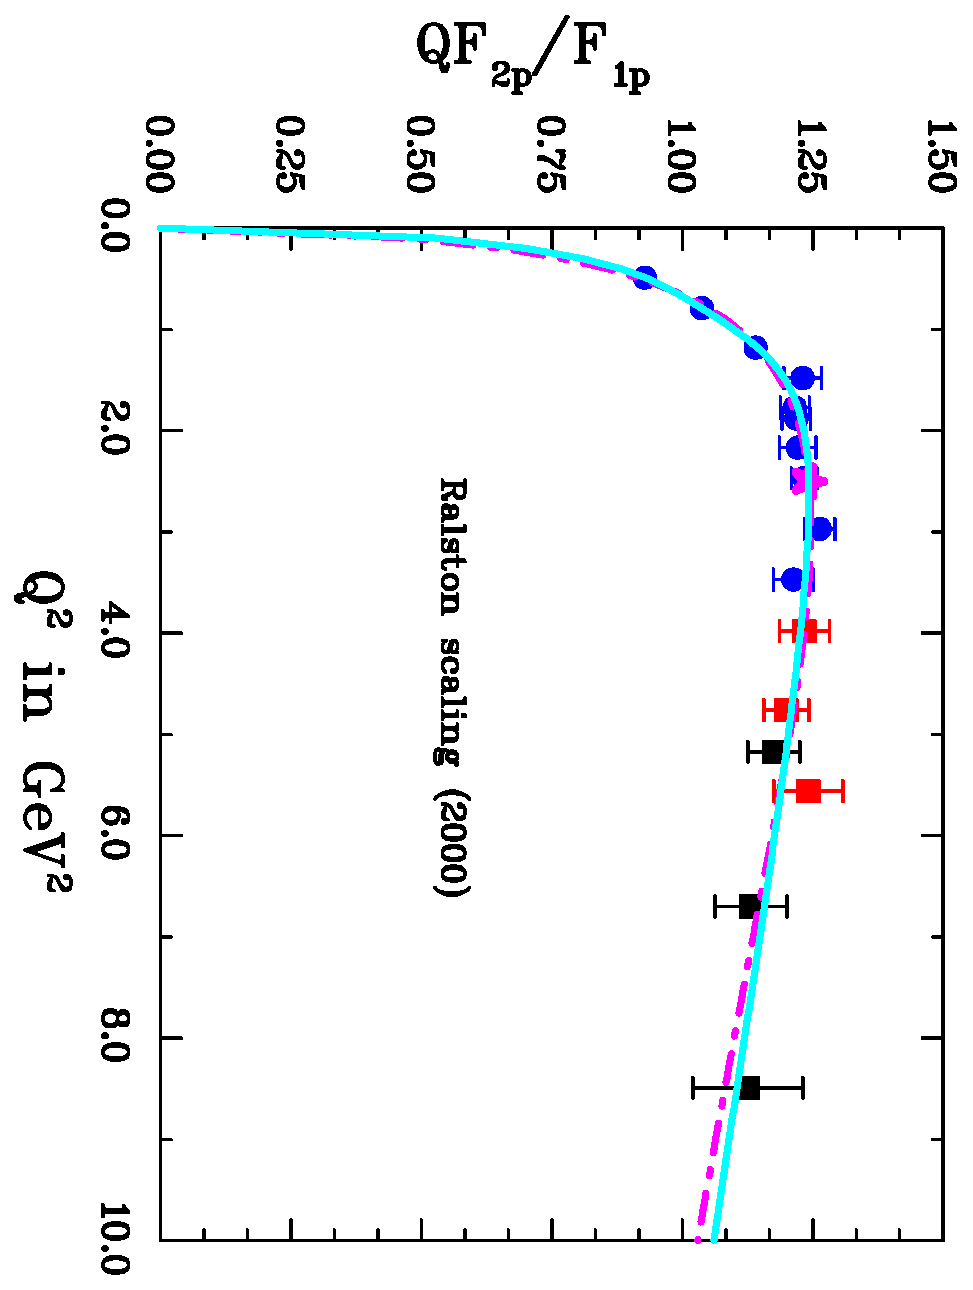
\includegraphics[angle=90]{qf2f1_gep3_colss.eps}
}
\caption{Behavior of the ratio $QF_2.F_1$ for the proton, as discussed by Ralston, \cite{jain}.}
\label{fig:pf2f1p}
\end{center}
\end{figure}

%%%%%%%%%%%%%%  Figure 14
\begin{figure}
\begin{center}
\resizebox{0.45\textwidth}{!}{%
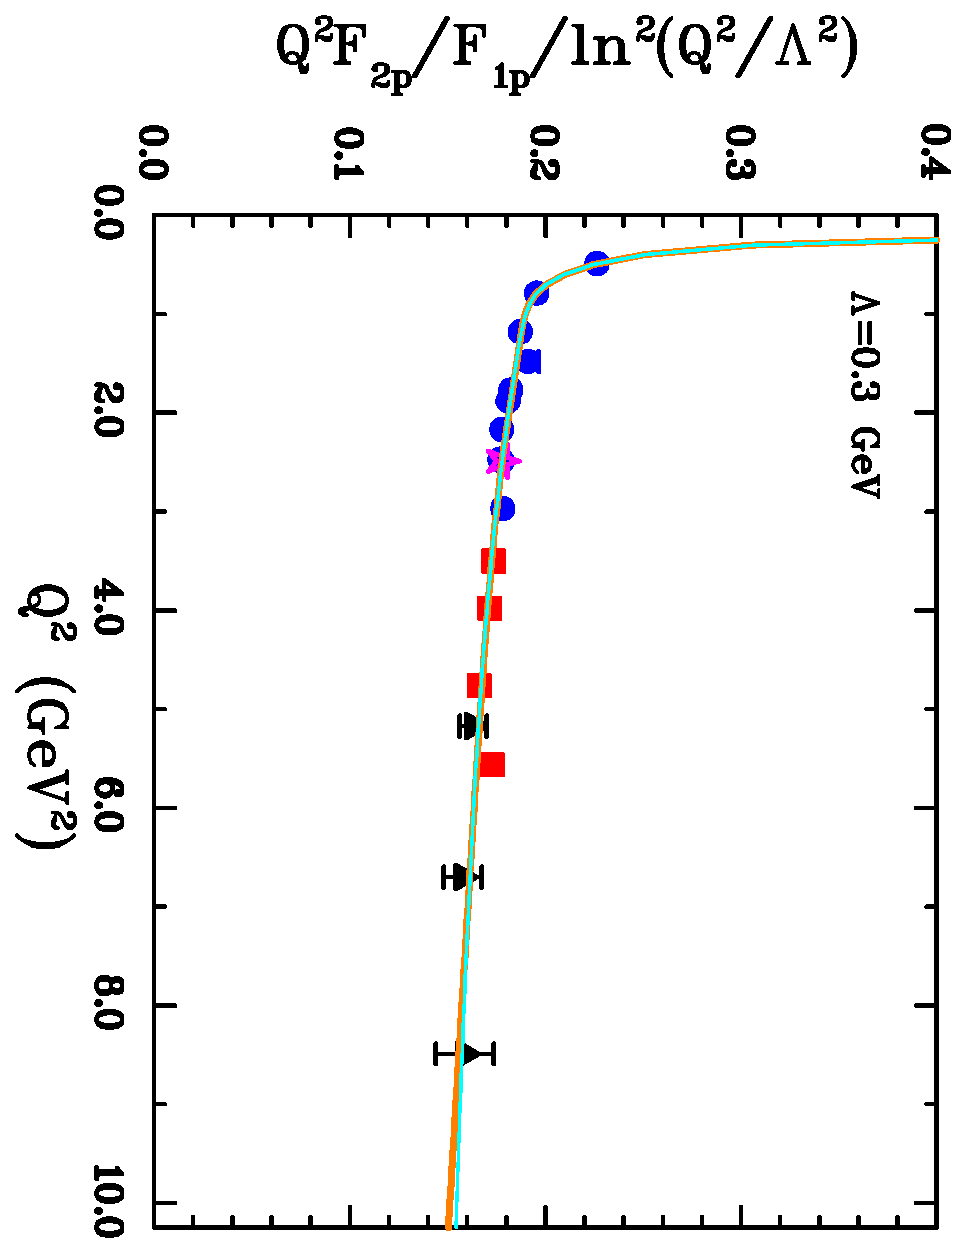
\includegraphics[angle=90]{q2f2f1_belitsky_nothss.eps}
}
\caption{Behavior of $Q^2F_2/F_1/ln^2(Q^2/\Lambda^2)$ as discussed by Belitsky \cite{belitsky:2002}.}
\label{fig:q2f2f1p_scal}
\end{center}
\end{figure}

%%%%%%%%%%%%%%%%%%% Figure 15
\begin{figure}
\begin{center}
\resizebox{0.45\textwidth}{!}{%
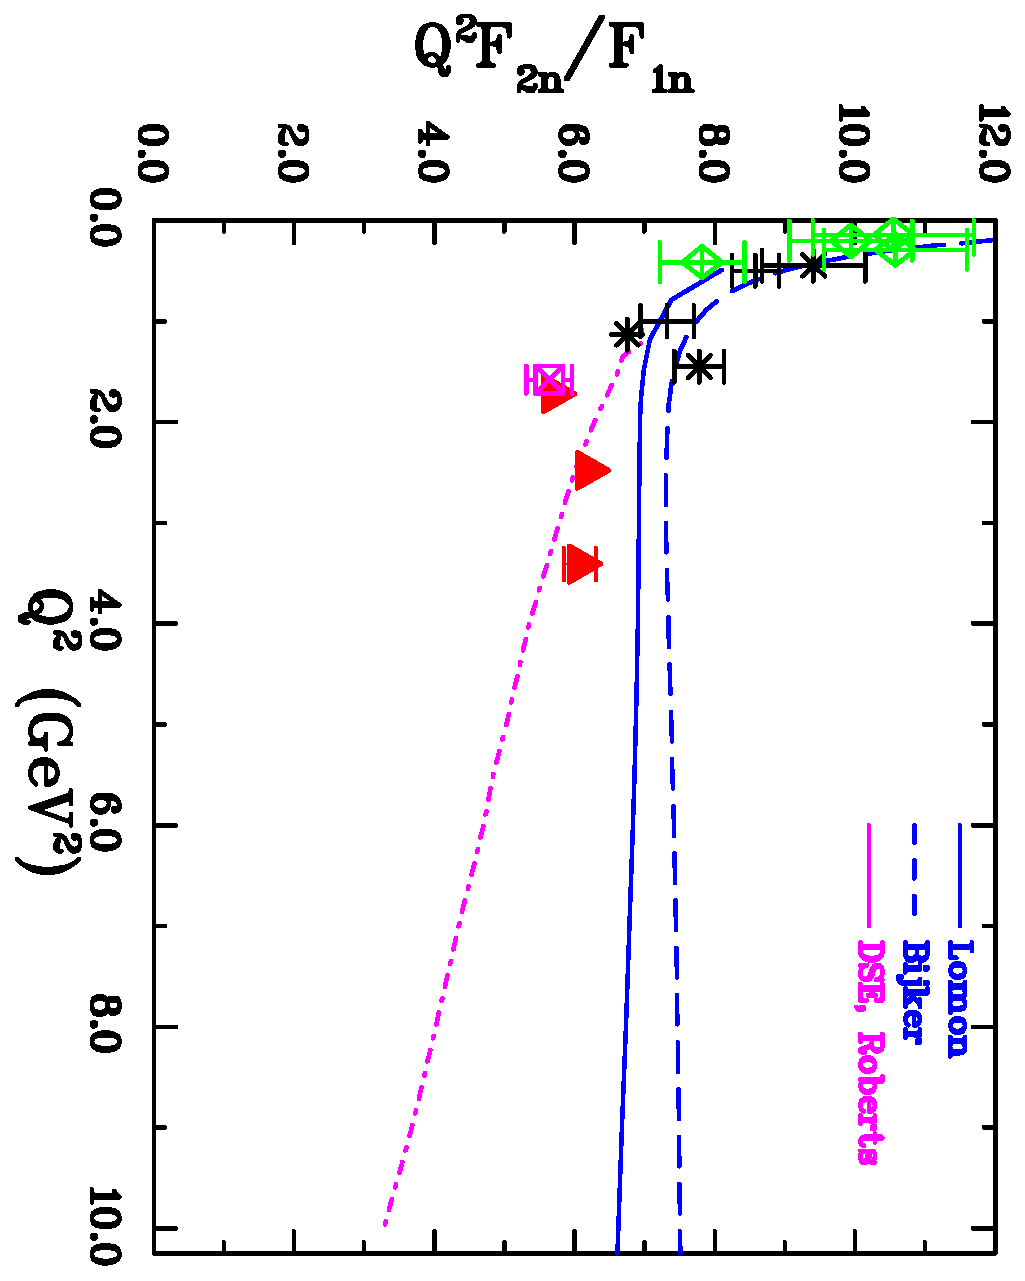
\includegraphics[angle=90]{q2f2f1_neutron_112311.eps}
}
\caption{Illustration of the current status on the asymptotic behavior of $Q^2F_2/F_1$ for the neutron; all data ;points from double polarization experiments. ``My Fit'' needs to be verified.}
\label{fig:pf2f1p_asymp}
\end{center}
\end{figure}

%%%%%%%%%%%%%%%%%%% Figure 16
\begin{figure}
\begin{center}
\resizebox{0.45\textwidth}{!}{%
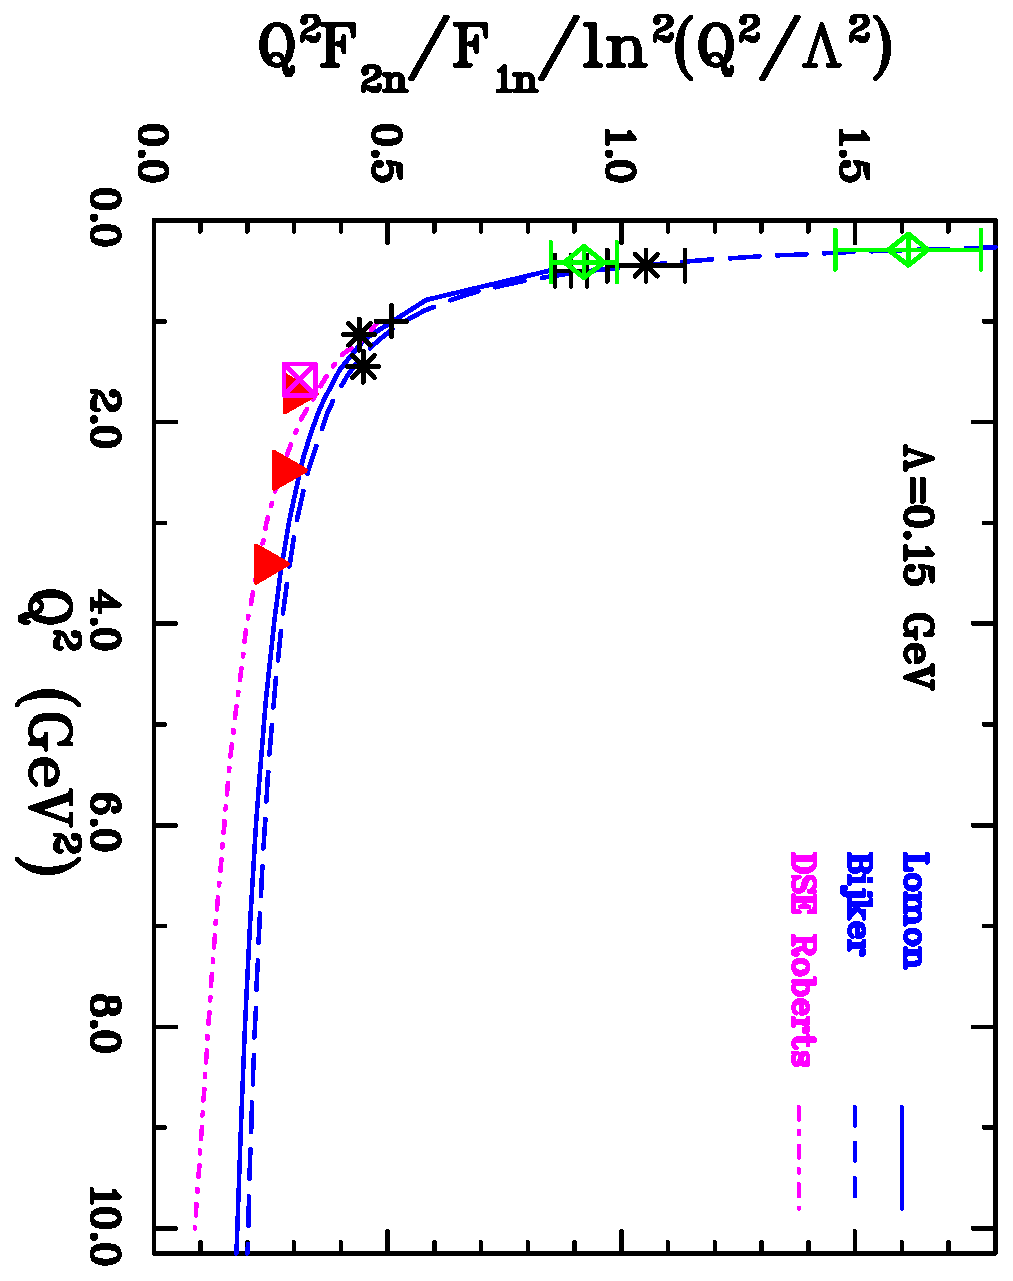
\includegraphics[angle=90]{q2f2f1_neutron_belitzky_052212.eps}
}
\caption{The Belitzky plot for the neutron}
\label{fig:nq2f2bel}
\end{center}
\end{figure}

%%%%%%%%%%%%%%added November 17, 2014


%%%
%\end{document}




